\documentclass[preprint,12pt,authoryear,nopreprintline]{elsarticle}

\usepackage[T1]{fontenc}
\usepackage[utf8]{inputenc}
\usepackage[margin=1in]{geometry}
\usepackage{amsmath,amssymb,amsthm,mathtools}
\usepackage{booktabs,multirow,array}
\usepackage{graphicx}
\usepackage{algorithm}
\usepackage{algpseudocode}
\usepackage{microtype}
\usepackage{xcolor}
\usepackage{url}
\usepackage[hidelinks]{hyperref}

\newtheorem{proposition}{Proposition}
\setlength{\emergencystretch}{2em}

\journal{Transportation Research Part C: Emerging Technologies}

\begin{document}

\begin{frontmatter}

\title{FreqDuet: Frequency-Separated and Turnaround-Budgeted Bi-Level Constrained Reinforcement Learning for Non-Stationary Urban Bus Corridors}

\author[aff1]{Anonymous Authors}
\address[aff1]{Submitted to Transportation Research Part C: Emerging Technologies}

\begin{abstract}
Real-time control on high-frequency urban bus corridors spans two coupled authorities: slow-clock terminal headway allocation ($15\text{--}60\text{ min}$) to match diurnal tidal demand waves under fixed vehicle pools and daily trip quotas, and stop-event vehicle holding ($5\text{--}25\text{ s}$) to suppress bunching and absorb localized boarding shocks. Existing analytical rules equalize raw gaps regardless of onboard passenger occupancy or non-stationary timetable transitions, while unconstrained hierarchical reinforcement learning (HRL) suffers from cross-band automatic passenger counting (APC) confounding and late-training fleet starvation when cumulative stop holding exhausts terminal turnaround slack. We propose \textbf{FreqDuet}, a frequency-separated, turnaround-budgeted bi-level constrained Soft Actor-Critic (SAC) framework operating strictly on causal APC and automatic vehicle location (AVL) observations. FreqDuet pairs a headway-normalized causal APC rate feed---eliminating concave log-rate Jensen bias under intermittent arrivals---with an online damped Fourier Recursive Least Squares (Harmonic-RLS) decomposer and persistent shock promotion gate, routing smooth low-frequency diurnal forecasts to an upper slow-clock Ensemble SAC planner (equipped with a Newell-consistent quota potential) and localized high-frequency positive innovations to a lower stop-event Constrained Ensemble SAC controller. A causal first-in-first-out (FIFO) Turnaround Budget Ledger translates scheduled opposite-direction launches and vehicle arrival-time projections into hard per-trip holding masks alongside a zero-hold-advantage critic and Lagrangian safety dual. Because all rewards and costs are formulated in estimator-free physical person-seconds, matched-dimension five-way observation ablations cleanly isolate the causal value of frequency-to-authority alignment. Across an empirical Fall~2025 Boston MBTA Route~111 weekday corridor reconstructed from GTFS and stop-level APC records ($9{,}330\text{ pax/day}$) and a high-load bimodal tidal corridor ($15{,}660\text{ pax/day}$), FreqDuet reduces passenger journey time by $14.32\text{ s/pax}$ and $14.02\text{ s/pax}$ over no-hold operations, by $45.34\text{ s/pax}$ and $48.78\text{ s/pax}$ over bilateral headway equalization, and by $9.59\text{ s/pax}$ over unseparated no-frequency HRL on empirical APC data, while sustaining monotonic $200$-episode stability and outperforming rolling economic MPC by $28.16\text{ s/pax}$ under corridor-wide congestion.
\end{abstract}

\begin{keyword}
public transit control \sep bus bunching \sep hierarchical reinforcement learning \sep constrained Markov decision process \sep frequency decomposition \sep turnaround slack
\end{keyword}

\end{frontmatter}

\section{Introduction}
\label{sec:intro}

Two decisions share the same scarce vehicle time on a high-frequency bus corridor. The dispatch planner can move scheduled departures toward periods of higher demand without adding daily trips. At a stop, holding can improve spacing, but it delays riders already on board and can postpone a vehicle's return for a trip in the opposite direction. A stop-level action that looks helpful on a headway metric need not be helpful to passengers or to the next terminal departure \citep{osuna1972control,daganzo2009headway,berrebi2018comparing}.

We study a fixed fleet circulating between two terminals. FreqDuet uses an upper policy to adjust a departure plan and a trip budget retention parameter every 15 minutes. A lower policy acts after a stop's boarding exchange. It can hold only within the remaining trip budget. The budget is based on a projection of which vehicles can cover upcoming departures, so it constrains actions without assuming that forecast return times will be realized. The upper and lower policies also use different summaries of a shared APC-derived signal: the upper policy emphasizes smooth directional demand and the lower policy emphasizes recent local departures from that trend.

The study makes three contributions:
\begin{enumerate}
  \item It specifies an executable joint dispatch and holding architecture under a fixed fleet and trip roster. An analytical two-gap model explains why unequal planned spacings, onboard load and future vehicle availability matter to the holding decision.
  \item It implements quota-aware dispatch and per-trip holding budgets in a discrete, two-level learning controller. The experiments compare the whole policy with fixed dispatch, two named headway feedback rules, a rolling dispatch heuristic, and other learned policies.
  \item It separates two empirical questions: whether joint control improves passenger outcomes relative to fixed dispatch, and whether the tested demand-feature representation improves a shared two-level controller. We evaluate paired simulated demand days and report training-seed sensitivity and the operating regimes where the comparison changes.
\end{enumerate}

The two nominal-corridor tests show shorter passenger journeys relative to no holding, mainly from less waiting, with some loss of arrival regularity and longer readiness delay. Comparisons with dynamic alternatives are more mixed. The MBTA-informed simulation supports a benefit from the tested demand features relative to a coarse APC feature block. The synthetic tidal corridor does not support the same conclusion. These distinctions matter when choosing between a joint learned controller and a simpler operating rule.

\section{Literature Review}
\label{sec:related}

\subsection{Analytical and Optimization-Based Bus Holding Control}
\label{sec:related_holding}

The instability of close-interval transit operations was first formalized by \citet{welding1957instability} and \citet{osuna1972control}, who showed that passenger waiting time scales with $1 + \mathrm{CV}^2(H)$, where $\mathrm{CV}^2(H) = \mathrm{Var}(H)/\mathbb{E}[H]^2$ denotes the squared coefficient of variation of vehicle headways. Early real-time control formulations leveraged emerging AVL data to cast stop-level holding as deterministic or stochastic rolling-horizon quadratic programs minimizing weighted passenger waiting and onboard delay \citep{eberlein2001holding,hickman2001analytic,sun2014models}. However, full corridor-wide mathematical programs with capacity constraints \citep{delgado2012much,sanchez2016realtime} require multi-step arrival predictions across all origin--destination pairs and solve mixed-integer or nonlinear programs at every stop event.

To obtain scalable, closed-form feedback laws, \citet{daganzo2009headway} introduced adaptive forward-headway holding, proving that linear feedback on deviations from a target headway eliminates bunching under mild perturbations. Subsequent extensions incorporated cooperative two-sided spacing using both predecessor and follower positions \citep{daganzo2011cooperation,bartholdi2012self}, virtual reference schedules \citep{xuan2011dynamic}, signalized corridor priority \citep{estrada2016bus}, overtaking and distributed boarding dynamics \citep{wu2017modelling}, predictive headway estimation \citep{andres2017predictive}, and dynamic bus substitution \citep{petit2018substitution}. In a comprehensive comparative evaluation, \citet{berrebi2018comparing} demonstrated that bilateral holding rules achieve strong headway regularity without requiring long-horizon predictions, establishing a widely adopted benchmark in transit operations \citep{cats2011impacts,cats2012guidelines}. Nevertheless, as highlighted in the synthesis of \citet{gkiotsalitis2021atstop}, purely headway-equalizing rules remain blind to onboard passenger occupancy, time-varying scheduled headway transitions, and terminal turnaround slack under finite fleets.

\subsection{Dynamic Timetabling and Fixed-Fleet Corridor Circulation}
\label{sec:related_dispatch}

On timescales of $15$--$60\text{ min}$, passenger demand along urban radial corridors exhibits pronounced directional asymmetry and peak-to-trough variation that cannot be addressed by stop-level holding around a static headway. \citet{newell1971dispatching} proved that when a fixed number of daily vehicle dispatches is allocated across a non-stationary arrival intensity $\Lambda(t)$ to minimize total passenger waiting time without capacity saturation, optimal dispatch frequency scales proportionally to $\sqrt{\Lambda(t)}$ (equivalently, target headway $H^\star(t) \propto \Lambda(t)^{-1/2}$). Modern automated fare collection and APC systems enable rich empirical characterization of these spatio-temporal demand profiles \citep{pelletier2011smart,furth2006service}.

Translating time-varying dispatch rates into executable corridor operations is constrained by vehicle circulation across both directions \citep{ibarra2015planning,ceder2016public}. \citet{gkiotsalitis2019robust} formulated robust timetable optimization subject to fleet size and regulatory layover bounds, showing that aggressive peak headway compression erodes terminal recovery time and amplifies trip-to-trip delay propagation. When real-time holding is deployed concurrently with dynamic dispatch on a fixed-pool corridor, the two authorities become tightly coupled through terminal inventory: every second of en-route holding directly consumes terminal layover slack prior to the vehicle's next opposite-direction trip. Existing optimization frameworks rarely coordinate real-time stop holding with dynamic quota-conserving headway allocation in closed loop without resorting to brittle centralized trajectory forecasts.

\subsection{Reinforcement Learning and Multi-Timescale Control in Transit}
\label{sec:related_rl}

Deep reinforcement learning has emerged as an attractive model-free alternative for real-time bus control under complex stochastic dwell and traffic dynamics. \citet{chen2016marl} and \citet{alesiani2018rl} pioneered multi-agent Q-learning and policy-gradient holding controllers on single-loop corridors. \citet{wang2020dynamic} introduced a multi-agent actor--critic framework with graph-structured vehicle interactions, later extending it to asynchronous event-driven execution \citep{wang2021asynchronous} and distributional risk-sensitive critics \citep{wang2023robust}. \citet{rodriguez2023cooperative} combined holding and stop-skipping in a cooperative DRL policy, while \citet{yu2024hierarchical} explored hierarchical multi-agent RL for bunching mitigation. Most recently, \citet{xu2025systematic} conducted a systematic benchmark of RL bus bunching configurations, cautioning that reward functions dominated by headway equalization frequently inflate in-vehicle travel times and fail to outperform simple analytical baselines on net passenger journey time when evaluated under realistic fleet constraints.

In parallel, the machine learning literature has established principles for temporal abstraction \citep{sutton1999between,nachum2018data}, off-policy maximum-entropy actor--critic learning \citep{haarnoja2018soft,christodoulou2019discrete,chen2021redq}, constrained MDPs via Lagrangian duality \citep{altman1999constrained,miryoosefi2019constraints,stooke2020responsive}, and multi-frequency control \citep{lee2020multiple,metelli2020persistence,holt2025evocontrol}. However, directly transplanting generic hierarchical RL to public transit fails for two domain-specific reasons: (i) temporal action abstraction alone does not prevent high-frequency APC sampling noise and localized demand spikes from corrupting upper-level timetable decisions, and (ii) unconstrained lower-level exploration systematically violates terminal turnaround feasibility on fixed-pool corridors.

\begin{table}[t]
\centering
\caption{Positioning of \texttt{FreqDuet} relative to representative transit control paradigms.}
\label{tab:literature_positioning}
\resizebox{\textwidth}{!}{%
\begin{tabular}{@{}lcccccc@{}}
\toprule
Study / Paradigm & Dynamic & Stop-Event & Demand Band & Fixed-Pool & Onboard-Load & Causal APC/AVL \\
 & Headway & Holding & Separation & Turnaround Cap & Journey Obj. & Identification \\
\midrule
\citet{daganzo2009headway} & -- & Forward & -- & -- & -- & \checkmark \\
\citet{berrebi2018comparing} & -- & Bilateral & -- & -- & -- & \checkmark \\
\citet{sanchez2016realtime} & -- & Rolling QP & -- & Soft / Open & \checkmark & Forecast-dep. \\
\citet{gkiotsalitis2019robust} & Offline / Per. & -- & -- & \checkmark & \checkmark & -- \\
\citet{wang2020dynamic,wang2023robust} & -- & MARL & -- & Ring / Uncap. & Partial & Raw state \\
\citet{yu2024hierarchical} & Regional HRL & MARL & -- & Uncapped & Headway-dom. & Raw state \\
\textbf{\texttt{FreqDuet} (Ours)} & \textbf{Slow SAC} & \textbf{CMDP SAC} & \textbf{LF$\to$U, HF$\to$L} & \textbf{Hard FIFO Mask} & \textbf{Exact Pax-s} & \textbf{4-Way Causal} \\
\bottomrule
\end{tabular}%
}
\end{table}

Table~\ref{tab:literature_positioning} summarizes how FreqDuet bridges these research streams. Unlike single-level holding controllers \citep{daganzo2009headway,berrebi2018comparing,wang2020dynamic} or unconstrained hierarchical RL \citep{yu2024hierarchical}, FreqDuet aligns online frequency-decomposed APC signals with the physical authority of each control layer while enforcing exact daily trip quotas and hard FIFO turnaround budgets under estimator-free passenger journey objectives.

\section{Problem Formulation}
\label{sec:problem}

\subsection{Fixed Fleet and Terminal Dispatch}
\label{sec:problem_corridor}

A bidirectional corridor has a physical fleet of $N_{\mathrm{fleet}}$ buses, capacity $C_{\mathrm{bus}}$, and a roster of $M_d$ trips in direction $d\in\{+,-\}$. Trips depart from one terminal and return to the other terminal's vehicle pool. The planner may revise uncommitted departure times $\tau_{d,m}^{\mathrm{sched}}$ and target headways $H_{d,m}$, but does not add or remove trips. The final planned departure in each direction is no earlier than the original final departure and the demand cutoff $T_{\mathrm{end}}$. We distinguish this planning constraint from completing the roster in the realized simulation.

A trip becomes eligible for dispatch when its revised scheduled time and minimum terminal separation permit it. It then waits if no vehicle is ready. The reported readiness delay is $D_{d,m}^{\mathrm{ready}}=\tau_{d,m}^{\mathrm{act}}-\tau_{d,m}^{\mathrm{elig}}$, where $\tau_{d,m}^{\mathrm{elig}}$ is the first eligible time. This is not delay from the original public timetable and excludes waiting before first eligibility. At intermediate stops a bus boards up to its remaining capacity. Its return time includes link travel, passenger-service dwell and discretionary holding:
\begin{equation}
  \tau^{\mathrm{ret}}_{v,m} = \tau^{\mathrm{act}}_{d,m} + T^{\mathrm{link}}_{v,m}
      + T^{\mathrm{dwell}}_{v,m} + \sum_s u_{v,m,s}.
  \label{eq:return_time}
\end{equation}
The simulator requires the vehicle to be available at the receiving terminal before reuse. The 20~s buffer used later in the ledger is a planning allowance, not a mandatory physical layover.

\subsection{Passenger and Regularity Metrics}
\label{sec:problem_metrics}

For the $|\mathcal{P}|$ passengers generated by the demand cutoff, restricted mean journey exposure $J_{\mathrm{pax}}$ is total waiting plus onboard person-time divided by $|\mathcal{P}|$. A passenger still waiting or riding at the evaluation cutoff contributes time accrued through that cutoff. We also report the fraction not served. The means do not condition on completing a journey.

For recorded nonterminal \emph{arrival} headways $h$, we report raw $\mathrm{CV}^2_{\mathrm{raw}}=\mathrm{Var}(h)/\mathbb{E}[h]^2$. Let $\mathcal{E}$ contain the observed headways and their active target headways $H$. Plan-normalized headway error and the excess-waiting-time (EWT) proxy are:
\begin{equation}
\begin{aligned}
  \mathrm{CV}^2_{\mathrm{plan}} &=
     \frac{1}{|\mathcal{E}|}\sum_{(h,H)\in\mathcal E}\left(\frac{h-H}{H}\right)^2,\\
  \mathrm{EWT} &= \frac{1}{|\mathcal{S}|}\sum_{(s,d)\in\mathcal{S}}
  \left[\frac{\sum_j h_{s,d,j}^2}{2\sum_j h_{s,d,j}} -
        \frac{\sum_j H_{s,d,j}^2}{2\sum_j H_{s,d,j}}\right],
\end{aligned}
\label{eq:plan_cv2_ewt}
\end{equation}
where $\mathcal{S}$ is the set of stop-direction groups with valid headways. EWT is relative to each controller's own plan, not a shared public timetable or a direct measure of actual passenger waits. The raw CV$^2$ does not remove intentional headway changes. Neither metric substitutes for the direct passenger outcome.

\subsection{A Plan-Consistent Two-Gap Holding Target}

\begin{proposition}[Plan-Consistent Non-Stationary Bilateral Holding Target]
\label{prop:nonstationary_target}
Suppose vehicle $v$ serving trip $(d,m)$ with planned headway $H_{\mathrm{own}} > 0$ completes boarding at stop $s$ with causal forward departure headway $g^{\mathrm{fwd}} \ge 0$ and same-time causal follower departure gap $g^{\mathrm{bwd}} \ge 0$, where the trailing vehicle serves trip $(d,m+1)$ with planned headway $H_{\mathrm{fol}} > 0$. Applying holding $u \in [0,\bar u]$ with $\bar u>0$ shifts the local gaps to $(g^{\mathrm{fwd}} + u,\, g^{\mathrm{bwd}} - u)$. Minimizing the local plan-normalized regularity loss
\begin{equation}
  \mathcal{L}_{\mathrm{reg}}(u) = \frac{1}{2}\left[\left(\frac{g^{\mathrm{fwd}} + u - H_{\mathrm{own}}}{H_{\mathrm{own}}}\right)^2 + \left(\frac{g^{\mathrm{bwd}} - u - H_{\mathrm{fol}}}{H_{\mathrm{fol}}}\right)^2\right]
  \label{eq:local_reg_loss}
\end{equation}
over $u \in [0, \bar{u}]$ yields the unique closed-form target
\begin{equation}
  u^\star = \mathrm{clip}\!\left(
    \frac{(g^{\mathrm{bwd}} - H_{\mathrm{fol}}) H_{\mathrm{fol}}^{-2} - (g^{\mathrm{fwd}} - H_{\mathrm{own}}) H_{\mathrm{own}}^{-2}}{H_{\mathrm{own}}^{-2} + H_{\mathrm{fol}}^{-2}},
    \, 0,\, \bar{u}
  \right).
  \label{eq:u_star_nonstationary}
\end{equation}
In particular, when $H_{\mathrm{own}} = H_{\mathrm{fol}}$, Eq.~\eqref{eq:u_star_nonstationary} reduces to the classical bilateral rule $u_{\mathrm{stat}}^\star = \mathrm{clip}(\frac{1}{2}(g^{\mathrm{bwd}} - g^{\mathrm{fwd}}), 0, \bar{u})$. However, when vehicles follow a non-stationary schedule perfectly ($g^{\mathrm{fwd}} = H_{\mathrm{own}}$, $g^{\mathrm{bwd}} = H_{\mathrm{fol}}$) with $H_{\mathrm{fol}} > H_{\mathrm{own}}$ (peak-to-off-peak transition), Eq.~\eqref{eq:u_star_nonstationary} yields $u^\star = 0$, whereas the stationary rule injects spurious holding $u_{\mathrm{stat}}^\star = \frac{1}{2}(H_{\mathrm{fol}} - H_{\mathrm{own}}) > 0$.
\end{proposition}

\begin{proof}
The objective $\mathcal{L}_{\mathrm{reg}}(u)$ in Eq.~\eqref{eq:local_reg_loss} is strictly convex in $u$ with second derivative $\mathcal{L}_{\mathrm{reg}}''(u) = H_{\mathrm{own}}^{-2} + H_{\mathrm{fol}}^{-2} > 0$. Setting the first derivative to zero gives
\begin{align*}
  &\frac{g^{\mathrm{fwd}} + u - H_{\mathrm{own}}}{H_{\mathrm{own}}^2} - \frac{g^{\mathrm{bwd}} - u - H_{\mathrm{fol}}}{H_{\mathrm{fol}}^2} = 0 \\
  &\iff u\bigl(H_{\mathrm{own}}^{-2} + H_{\mathrm{fol}}^{-2}\bigr) = (g^{\mathrm{bwd}} - H_{\mathrm{fol}}) H_{\mathrm{fol}}^{-2} - (g^{\mathrm{fwd}} - H_{\mathrm{own}}) H_{\mathrm{own}}^{-2}.
\end{align*}
Projecting the unconstrained minimizer onto the compact interval $[0, \bar{u}]$ yields Eq.~\eqref{eq:u_star_nonstationary}. Substituting $H_{\mathrm{own}} = H_{\mathrm{fol}} = H$ cancels $H^{-2}$ and cancels $\pm H$ in the numerator, yielding $\frac{1}{2}(g^{\mathrm{bwd}} - g^{\mathrm{fwd}})$. Substituting $g^{\mathrm{fwd}} = H_{\mathrm{own}}$ and $g^{\mathrm{bwd}} = H_{\mathrm{fol}}$ makes the numerator identically zero, so $u^\star = 0$, whereas $\frac{1}{2}(g^{\mathrm{bwd}} - g^{\mathrm{fwd}}) = \frac{1}{2}(H_{\mathrm{fol}} - H_{\mathrm{own}}) > 0$ whenever $H_{\mathrm{fol}} > H_{\mathrm{own}}$.
\end{proof}

\subsection{Local Waiting Savings and the Limits of Turnaround Pricing}
\label{sec:problem_osuna}

Under a constant arrival rate $\Lambda$ (passengers per second), no capacity limit and rigid shifts on a downstream two-gap segment, the expected waiting saved by holding $u$ is
\begin{equation}
  \Delta W(u)=\Lambda u(g^{\mathrm{bwd}}-g^{\mathrm{fwd}}-u).
  \label{eq:osuna_turnaround_delta}
\end{equation}
This follows by subtracting the squared-gap waiting cost after holding from that before holding \citep{osuna1972control}. The local onboard cost is $L^{\mathrm{on}}u$. When targets differ, the controller instead uses a plan-aware \emph{proxy} for the first term:
\begin{equation}
  G(u)=\widehat{\Lambda}^{\mathrm{ds}}\frac{H_{\mathrm{own}}+H_{\mathrm{fol}}}{2}u
  \left[\frac{g^{\mathrm{bwd}}}{H_{\mathrm{fol}}}-\frac{g^{\mathrm{fwd}}}{H_{\mathrm{own}}}
  -\frac{u}{2}\!\left(\frac{1}{H_{\mathrm{own}}}+\frac{1}{H_{\mathrm{fol}}}\right)\right].
  \label{eq:normalized_hold_proxy}
\end{equation}
It reduces to Eq.~\eqref{eq:osuna_turnaround_delta} for equal headway targets with $\Lambda=\widehat{\Lambda}^{\mathrm{ds}}$. With unequal targets, capacity constraints or state-dependent dwell, it is not the causal change in system-wide waiting.

Turnaround effects depend on future departures. For illustration, if the same vehicle is required for the next dispatch, a hold beyond its actual slack can delay that dispatch. Whether the resulting net waiting cost is large also depends on the next gap. With constant arrivals, initially equal gaps $H$, and a single dispatch delayed by $\delta<H$ while its neighbors stay fixed, gaps become $H+\delta$ and $H-\delta$, and the added waiting across both gaps is $\Lambda\delta^2$. Other ready vehicles may absorb the delay entirely. We therefore use predicted slack to limit holds, and measure passenger and vehicle consequences in simulation rather than assuming a lower bound on spillover.

\section{Methodology: The \texttt{FreqDuet} Architecture}
\label{sec:method}

Figure~\ref{fig:architecture} illustrates the closed-loop \texttt{FreqDuet} framework. The architecture comprises four tightly integrated modules: (i) a causal headway-normalized APC rate feed and online Harmonic-RLS frequency decomposer with persistent shock promotion; (ii) an upper slow-clock ($\Delta T_U = 900\text{ s}$) Ensemble SAC planner with exact daily quota conservation; (iii) a causal FIFO Turnaround Budget Ledger updated every $60\text{ s}$; and (iv) a lower stop-event Constrained Ensemble SAC controller equipped with hard turnaround action masking and a zero-hold-advantage critic.

\begin{figure}[t]
  \centering
  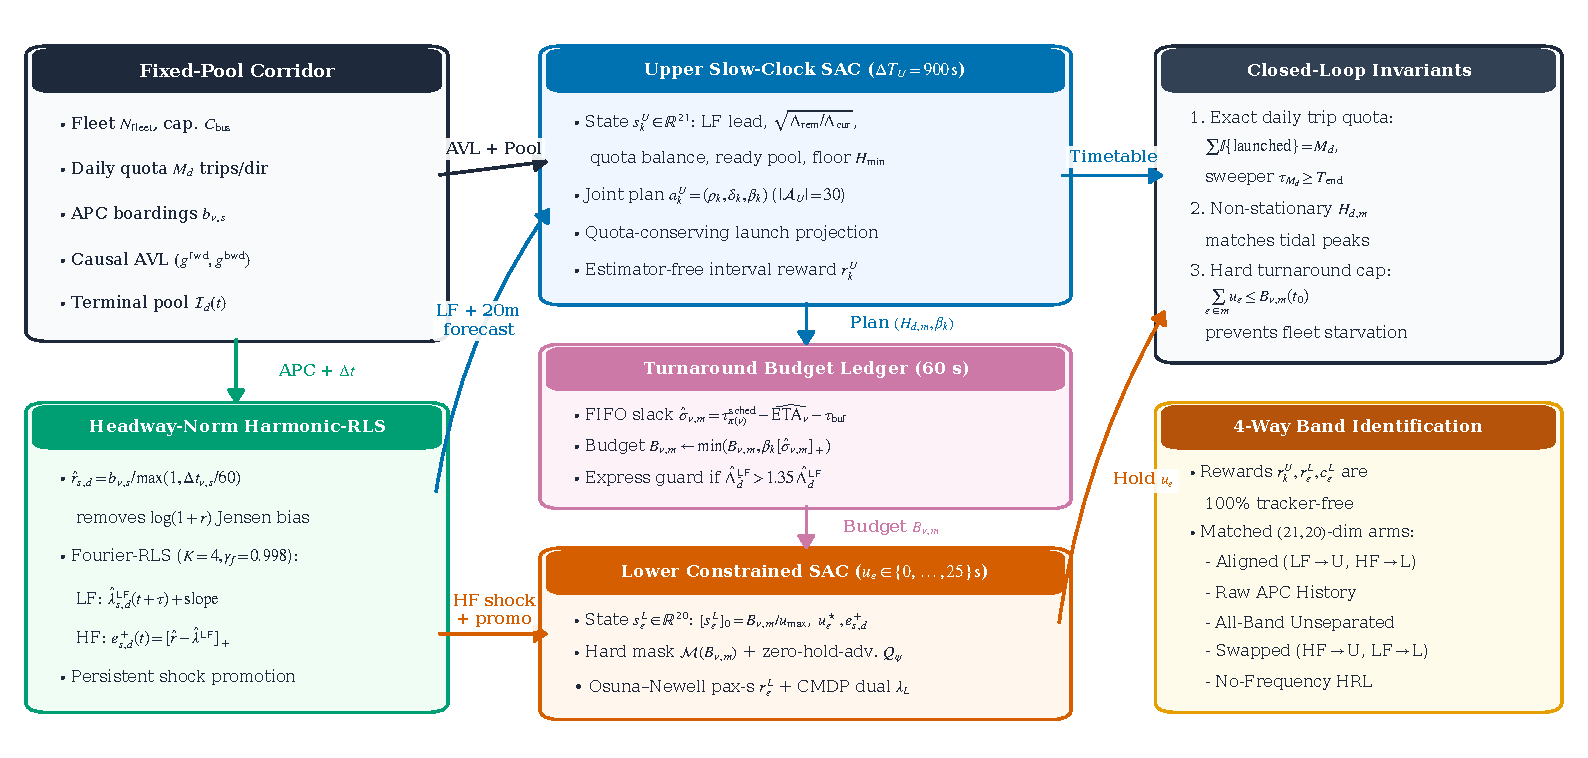
\includegraphics[width=\textwidth]{figures/fig1_architecture.pdf}
  \caption{Overview of the \texttt{FreqDuet} bi-level frequency-separated and turnaround-budgeted constrained reinforcement learning architecture. Low-frequency diurnal level, slope, and $20\text{-min}$ harmonic forecasts guide global quota-conserving timetable allocation, while localized high-frequency positive innovations guide stop-event holding within a hard FIFO turnaround slack budget.}
  \label{fig:architecture}
\end{figure}

\subsection{Causal Headway-Normalized APC Decomposition and Shock Promotion}
\label{sec:method_frequency}

In deployable APC/AVL systems, stop-level passenger demand is not observed continuously; rather, boarding count $b_{v,s}$ is recorded only when vehicle $v$ completes service at stop $(s,d)$ at time $t_e$. If headways average $6\text{ min}$ and raw $1\text{-min}$ APC bins $[0,0,0,0,0,b_{v,s}]$ are fed directly into a concave log-rate filter $y_t = \log(1 + r_t)$, Jensen's inequality ($\frac{1}{6}\log(1 + 6\lambda) \ll \log(1 + \lambda)$) depresses the estimated low-frequency arrival rate by more than $3\times$ (Figure~\ref{fig:corridors}c). Moreover, on the first vehicle visit to stop $(s,d)$ at $t_e$, passengers have accumulated since service opening $t = 0$, not over a nominal headway.

To obtain an unbiased, strictly causal arrival-rate stream, \texttt{FreqDuet} computes the \emph{headway-normalized causal APC rate} upon each boarding completion event $e = (v, s, d, t_e)$:
\begin{equation}
  \begin{aligned}
  \Delta t_e &=
  \begin{cases}
    \mathrm{clip}(h^{\mathrm{arr}}_e,\, 60,\, 1800), & \text{if } (s,d) \text{ has a prior arrival event}, \\
    \mathrm{clip}(\max(60,\, t_e),\, 60,\, 1800), & \text{on the first daily visit to } (s,d),
  \end{cases} \\
  \tilde{b}_e &= b_{v,s} \bigl(1 + 0.15\,\mathbb{I}\{L^{\mathrm{on}}_e = C_{\mathrm{bus}}\}\bigr),
  \end{aligned}
  \label{eq:apc_headway_norm}
\end{equation}
where $h^{\mathrm{arr}}_e$ is the realized arrival headway at $(s,d)$ and the factor $1.15$ provides a conservative causal censoring correction when the departing vehicle reaches full capacity $C_{\mathrm{bus}}$. The instantaneous rate $r^{\mathrm{inst}}_e = 60\,\tilde{b}_e / \Delta t_e$ ($\text{pax/min}$) updates the held stop rate via causal exponential smoothing $\hat{r}_{s,d}(t_e) \leftarrow 0.75\,r^{\mathrm{inst}}_e + 0.25\,\hat{r}_{s,d}(t_e^-)$, which is sampled at $1\text{-min}$ bin closures $n = \lfloor t / 60 \rfloor$.

At each $1\text{-min}$ bin $n$, an online damped Fourier Recursive Least Squares (Harmonic-RLS) estimator models log-intensity $y_{s,d}[n] = \log(1 + \hat{r}_{s,d}[n])$ over harmonic basis $\phi(n) \in \mathbb{R}^{2K+1}$ ($K = 4$, fundamental period $P = 50{,}400\text{ s}$):
\begin{equation}
  \phi(n) = \bigl[1,\, \cos(\omega n),\, \sin(\omega n),\, \dots,\, \cos(K\omega n),\, \sin(K\omega n)\bigr]^\top,
  \qquad
  \omega = \frac{2\pi \cdot 60}{P}.
  \label{eq:fourier_basis}
\end{equation}
Initialized from historical diurnal prior $(\theta_{s,d}[0], P_{s,d}[0] = \sigma_0^2 I)$ with $\sigma_0^2 = 0.35$ and forgetting factor $\gamma_f = 0.998$, the parameter vector updates causally via
\begin{equation}
  \kappa_{s,d}[n] = \frac{P_{s,d}[n-1]\phi(n)}{\gamma_f + \phi(n)^\top P_{s,d}[n-1]\phi(n)},
  \quad
  \theta_{s,d}[n] = \theta_{s,d}[n-1] + \kappa_{s,d}[n]\bigl(y_{s,d}[n] - \phi(n)^\top \theta_{s,d}[n-1]\bigr),
  \label{eq:rls_update}
\end{equation}
with $P_{s,d}[n] = \gamma_f^{-1}(I - \kappa_{s,d}[n]\phi(n)^\top)P_{s,d}[n-1]$. Inverting the log-link yields the causal low-frequency rate $\hat{\lambda}^{\mathrm{LF}}_{s,d}[n] = [\exp(\phi(n)^\top \theta_{s,d}[n]) - 1]_+$, the $\tau$-bin causal forecast $\hat{\lambda}^{\mathrm{LF}}_{s,d}[n+\tau] = [\exp(\phi(n+\tau)^\top \theta_{s,d}[n]) - 1]_+$ ($\tau = 20\text{ min}$), the instantaneous LF slope $\dot{\hat{\lambda}}^{\mathrm{LF}}_{s,d}[n]$, and the high-frequency positive shock residual and shock energy:
\begin{equation}
  e^{+}_{s,d}[n] = \bigl[\hat{r}_{s,d}[n] - \hat{\lambda}^{\mathrm{LF}}_{s,d}[n]\bigr]_+,
  \qquad
  E^{\mathrm{HF}}_{s,d}[n] = (1 - \alpha_E) E^{\mathrm{HF}}_{s,d}[n-1] + \alpha_E \bigl(\hat{r}_{s,d}[n] - \hat{\lambda}^{\mathrm{LF}}_{s,d}[n]\bigr)^2.
  \label{eq:hf_residual}
\end{equation}
Finally, a \emph{persistent shock promotion gate} distinguishes transient $1$--$2\text{ bus}$ boarding bursts from sustained regime shifts (such as unscheduled $1\text{-h}$ peak shifts). Only when $e^{+}_{s,d}$ exceeds $1.25$ standard deviations across at least $55\%$ of a trailing $10\text{-min}$ window (subject to a $15\text{-min}$ cooldown) does the tracker apply an accelerated gain ($\eta_{\mathrm{promo}} = 0.16$) to promote the persistent residual into the LF level $\hat{\lambda}^{\mathrm{LF}}_{s,d}$, while passing a normalized promotion age indicator to the lower controller.

\subsection{Upper Slow-Clock Quota-Conserving Ensemble SAC}
\label{sec:method_upper}

At slow-clock epochs $t_k = k \Delta T_U$ ($\Delta T_U = 900\text{ s}$), the upper controller observes a $21$-dimensional state vector $s^U_k = [x^{\mathrm{ops}}_k;\, z^{\mathrm{U}}_k] \in \mathbb{R}^{21}$. The $13$-dimensional operational core $x^{\mathrm{ops}}_k$ encodes diurnal phase $(\sin\varphi_k, \cos\varphi_k)$, remaining day fraction, directional remaining trip-quota balances, remaining quota-available headways $(H^{\mathrm{avail}}_+, H^{\mathrm{avail}}_-)$, normalized terminal ready counts $(|\mathcal{I}_+|/N_{\mathrm{fleet}}, |\mathcal{I}_-|/N_{\mathrm{fleet}})$, active on-route fleet fraction, dynamic cycle floor $H_{\min}(t_k)$, recent holding budget utilization, and realized readiness delay from the preceding $900\text{ s}$ interval. Under \texttt{FreqDuet}'s aligned routing, the $8$-dimensional demand block $z^{\mathrm{U}}_k$ supplies directional LF current rates, $20\text{-min}$ lead LF rates $\hat{\Lambda}^{\mathrm{LF}}_d = 0.3\sum_s \hat{\lambda}^{\mathrm{LF}}_{s,d}[n] + 0.7\sum_s \hat{\lambda}^{\mathrm{LF}}_{s,d}[n+20]$, directional LF slopes, Newell's root-intensity ratio $\mathbb{E}_{n'>n}[\sqrt{\hat{\Lambda}^{\mathrm{LF}}[n']}]/\sqrt{\hat{\Lambda}^{\mathrm{LF}}[n]}$ \citep{newell1971dispatching}, and directional LF tidal asymmetry $(\hat{\Lambda}^{\mathrm{LF}}_+ - \hat{\Lambda}^{\mathrm{LF}}_-)/(\hat{\Lambda}^{\mathrm{LF}}_+ + \hat{\Lambda}^{\mathrm{LF}}_-)$.

The upper policy $\pi_\theta(a^U_k \mid s^U_k)$ selects from $|\mathcal{A}_U| = 30$ discrete joint plans $a^U_k = (\rho_k, \delta_k, \beta_k)$ formed by the Cartesian product of loop headway compression factor $\rho_k \in \{0.78, 0.89, 1.00, 1.12, 1.24\}$, directional headway tilt $\delta_k \in \{-36, 0, +36\}\text{ s}$, and turnaround budget retention ratio $\beta_k \in \{0.50, 0.90\}$. Desired active-window headways incorporate an inventory guard $g_d(t_k) = \mathrm{clip}(0.55 + 0.35(|\mathcal{I}_d(t_k)| - |\mathcal{I}_{\bar{d}}(t_k)|),\, 0.15,\, 1)$ that suppresses aggressive directional tilting when terminal vehicle stock is depleted:
\begin{equation}
  H^{\mathrm{des}}_d(t_k) = \mathrm{clip}\!\Bigl(H^{\mathrm{avail}}_d(t_k)\,\rho_k + \mathrm{sgn}(d)\,\delta_k\,g_d(t_k),\, H_{\min}(t_k),\, H_{\max}\Bigr),
  \label{eq:desired_headway}
\end{equation}
where $H_{\min}(t_k)$ relaxes down to $0.85\,(\tilde{T}^{\mathrm{run}}_+ + \tilde{T}^{\mathrm{run}}_- + 40)/N_{\mathrm{fleet}}$ when terminal buffer stock $|\mathcal{I}_+| + |\mathcal{I}_-| \ge 3$ and tightens to $0.97$ of steady-state cycle headway when $|\mathcal{I}_+| + |\mathcal{I}_-| \le 1$.

To project $H^{\mathrm{des}}_d(t_k)$ onto the $K^{\mathrm{rem}}_d$ unlaunched mutable trips without violating Eq.~\eqref{eq:quota_sweeper_invariants}, let $\tau^{\mathrm{anc}}_d$ denote the last committed launch time and $S^{\mathrm{rem}}_d = \max(\tau^{\mathrm{base}}_{d,M_d}, T_{\mathrm{end}}) - \tau^{\mathrm{anc}}_d$ the remaining service span. Partitioning $K^{\mathrm{rem}}_d = K^{\mathrm{win}}_d + K^{\mathrm{tail}}_d$ into $K^{\mathrm{win}}_d = \min(K^{\mathrm{rem}}_d - 1, \max(2, \mathrm{round}(W_{\mathrm{act}}/H^{\mathrm{des}}_d)))$ near-term trips ($W_{\mathrm{act}} = 1800\text{ s}$) and $K^{\mathrm{tail}}_d$ tail trips with capacity-safe tail bounds $[T_{\min}, T_{\max}] = [255, 445]\text{ s}$, the executable active headway $H^{\mathrm{act}}_d$ and compensating tail headway $H^{\mathrm{tail}}_d$ are computed in closed form:
\begin{equation}
  \begin{aligned}
  H^{\mathrm{lo}}_d &= \max\!\Bigl(H_{\min},\, \frac{S^{\mathrm{rem}}_d - K^{\mathrm{tail}}_d T_{\max}}{K^{\mathrm{win}}_d},\, t_k + 1 - \tau^{\mathrm{anc}}_d\Bigr), \quad
  H^{\mathrm{hi}}_d = \min\!\Bigl(H_{\max},\, \frac{S^{\mathrm{rem}}_d - K^{\mathrm{tail}}_d T_{\min}}{K^{\mathrm{win}}_d}\Bigr), \\
  H^{\mathrm{act}}_d &= \mathrm{clip}\bigl(H^{\mathrm{des}}_d,\, H^{\mathrm{lo}}_d,\, H^{\mathrm{hi}}_d\bigr), \qquad
  H^{\mathrm{tail}}_d = \frac{S^{\mathrm{rem}}_d - K^{\mathrm{win}}_d H^{\mathrm{act}}_d}{K^{\mathrm{tail}}_d},
  \end{aligned}
  \label{eq:quota_projection}
\end{equation}
with uniform span fallback $H^{\mathrm{act}}_d = H^{\mathrm{tail}}_d = \max(T_{\min}, S^{\mathrm{rem}}_d / K^{\mathrm{rem}}_d)$ whenever $H^{\mathrm{lo}}_d > H^{\mathrm{hi}}_d$, and final sweeper trip $M_d$ pinned to $\max(\tau^{\mathrm{sched}}_{d,M_d-1} + H^{\mathrm{tail}}_d, \max(\tau^{\mathrm{base}}_{d,M_d}, T_{\mathrm{end}}))$.

To resolve long-horizon credit assignment across all $52$ daily slow-clock epochs without biasing the undiscounted passenger journey objective, we introduce a terminal-vanishing potential function $\Phi(s^U_k) = -\sum_{d \in \{+,-\}} \frac{1}{2}\bar{\lambda}_{\mathrm{dir}} S^{\mathrm{rem}}_d(t_k) H^{\mathrm{avail}}_d(t_k)$, where $\bar{\lambda}_{\mathrm{dir}} = P_{\mathrm{prior}}/(2 T_{\mathrm{end}})$ is the static nominal directional arrival rate and $\Phi(s_{\mathrm{term}}) = 0$. Over interval $[t_k, t_{k+1})$, the upper reward is:
\begin{equation}
  \begin{aligned}
  r^U_k &= \frac{-(W^{\mathrm{wait}}_k + W^{\mathrm{hold}}_k) + \gamma_U \Phi(s^U_{k+1}) - \Phi(s^U_k)}{360\,P_{\mathrm{ref}}} \\
        &\quad - 0.08\,\frac{\mathrm{clip}(\mathrm{EWT}_k, -20, 120)}{60}
               - 0.16\,\frac{\mathrm{clip}(\bar{D}^{\mathrm{ready}}_k, 0, 240)}{60}.
  \end{aligned}
  \label{eq:upper_reward}
\end{equation}
Because $\Phi(s^U_0)$ is policy-invariant and $\Phi(s_{\mathrm{term}}) = 0$, potential shaping preserves exact global optimality while immediately pricing quota depletion: differentiating $\frac{1}{2}\lambda_d(t)\Delta T_U H^{\mathrm{act}}_d - [\Phi(s^U_{k+1}) - \Phi(s^U_k)]$ with respect to $H^{\mathrm{act}}_d$ yields the first-order condition $H^{\mathrm{act},\star}_d(t) = H^{\mathrm{avail}}_d \sqrt{\bar{\lambda}_{\mathrm{dir}}/\lambda_d(t)}$, recovering \citet{newell1971dispatching}'s square-root dispatching law while naturally centering $r^U_k$ around zero. Furthermore, because a dispatched bus requires $35\text{--}75\text{ min}$ to complete a corridor round trip, we train $\{Q^U_{\phi_i}\}_{i=1}^{6}$ ($\gamma_U = 0.996$) using exact $N_U = 6$-step ($90\text{-min}$) Bellman backups with pessimistic LCB targets ($\beta_{\mathrm{LCB}} = -1.0$) \citep{haarnoja2018soft,christodoulou2019discrete,chen2021redq}.

\subsection{Causal Turnaround Budget Ledger}
\label{sec:method_ledger}

Every $60\text{ s}$ and upon any vehicle launch, the \emph{Turnaround Budget Ledger} translates the active timetable and upper retention tier $\beta_k \in \{0.50, 0.90\}$ into per-trip remaining holding budgets $B_{v,m}(t)$ without future oracle knowledge. For each direction $\bar{d}$, the ledger constructs the causal supply set of vehicles that will feed terminal $s_{\bar{d},0}$: (i) vehicles already idle at $s_{\bar{d},0}$ with ready time $\max(t, \tau^{\mathrm{ret}}_v + 1)$, and (ii) vehicles currently en route in direction $d$ at normalized corridor progress $\tilde{p}_v = d^{\mathrm{trav}}_v / L_d \in [0, 1]$, whose causal opposite-terminal ready ETA is
\begin{equation}
  \widehat{\mathrm{ETA}}_v(t) = t + (1 - \tilde{p}_v)\,\tilde{T}^{\mathrm{run}}_d(t) + h^{\mathrm{rem}}_v + w^{\mathrm{rem}}_v + 1,
  \label{eq:ledger_eta}
\end{equation}
where $h^{\mathrm{rem}}_v$ and $w^{\mathrm{rem}}_v$ are residual in-progress stop holding and dwell times. Sorting the supply set by $\widehat{\mathrm{ETA}}_v(t)$ and matching it in FIFO order against the sorted unlaunched schedule $\{\tau^{\mathrm{sched}}_{\bar{d},m'}\}$ assigns each active en-route trip $(v,m)$ to its paired opposite-direction launch $\pi(v,m)$ with projected turnaround slack $\hat{\sigma}_{v,m}(t) = \tau^{\mathrm{sched}}_{\pi(v,m)} - \widehat{\mathrm{ETA}}_v(t) - \tau_{\mathrm{buf}}$ ($\tau_{\mathrm{buf}} = 20\text{ s}$).

To prevent deadheading starvation during sharp tidal asymmetries, when opposite-direction LF demand dominates own-direction LF demand ($\hat{\Lambda}^{\mathrm{LF}}_{\bar{d}} > 1.35\,\hat{\Lambda}^{\mathrm{LF}}_d$) and $\hat{\sigma}_{v,m}(t) < 75\text{ s}$, the ledger activates a \emph{backhaul express guard}, tightening the proposed budget cap:
\begin{equation}
  B^{\mathrm{prop}}_{v,m}(t) =
  \begin{cases}
    \mathrm{clip}\bigl(0.40\,\beta_k\,[\hat{\sigma}_{v,m}(t)]_+,\, 0,\, 30\text{ s}\bigr), & \text{if } \hat{\Lambda}^{\mathrm{LF}}_{\bar{d}} > 1.35\,\hat{\Lambda}^{\mathrm{LF}}_d \text{ and } \hat{\sigma}_{v,m}(t) < 75\text{ s}, \\
    \mathrm{clip}\bigl(\beta_k\,[\hat{\sigma}_{v,m}(t)]_+,\, 0,\, 85\text{ s}\bigr), & \text{otherwise}.
  \end{cases}
  \label{eq:budget_proposal}
\end{equation}
Remaining trip budget updates monotonically via $B_{v,m}(t) \leftarrow \min(B_{v,m}(t^-),\, B^{\mathrm{prop}}_{v,m}(t))$ and is debited immediately upon every stop-level hold: $B_{v,m}(t^+) \leftarrow \max(0,\, B_{v,m}(t) - u_e)$. Thus cumulative holding along trip $(v,m)$ can never exceed available turnaround slack.

\subsection{Lower Hard-Masked Zero-Hold-Advantage Constrained SAC}
\label{sec:method_lower}

Whenever vehicle $v$ finishes passenger boarding at intermediate stop $s \in \{1, \dots, S_d-1\}$, the lower agent observes a $20$-dimensional state $s^L_e = [x^{\mathrm{loc}}_e;\, z^{\mathrm{L}}_e] \in \mathbb{R}^{20}$ and selects a discrete holding duration $u_e \in \mathcal{A}_L = \{0, 5, 10, 15, 20, 25\}\text{ s}$ ($u_{\max} = 25\text{ s}$). Critically, feature zero is defined as the normalized budget limit ratio $[s^L_e]_0 = \min(u_{\max}, B_{v,m}(t_e)) / u_{\max} \in [0, 1]$, followed by $15$ causal operational features (remaining trip budget, per-remaining-stop budget allowance, turnaround slack $\hat{\sigma}_{v,m}$, opposite-terminal overdue launch indicator, relative forward and backward gaps $(g^{\mathrm{fwd}} - H_{\mathrm{own}})/H_{\mathrm{own}}$ and $(g^{\mathrm{bwd}} - H_{\mathrm{fol}})/H_{\mathrm{fol}}$, two-sided AVL validity flag, analytical plan-consistent target $u^\star_e / u_{\max}$ from Proposition~\ref{prop:nonstationary_target}, own and follower planned headways, onboard load ratio $L^{\mathrm{on}}_e/C_{\mathrm{bus}}$, pass-up count, route progress, and diurnal phase). Under aligned frequency routing, the $4$-dimensional band block $z^{\mathrm{L}}_e$ supplies normalized local HF shock $e^{+}_{s,d}/\max(\hat{\lambda}^{\mathrm{LF}}_{s,d}, 0.5)$, local HF shock RMS $\sqrt{E^{\mathrm{HF}}_{s,d}}/\max(\hat{\lambda}^{\mathrm{LF}}_{s,d}, 0.5)$, maximum HF shock over the next two downstream stops, and local promotion age.

Three structural mechanisms stabilize lower-level learning across hundreds of training episodes:
\begin{enumerate}
  \item \textbf{Differentiable hard budget masking:} Directly inside the categorical policy network $\pi_\omega(u \mid s^L_e)$, action logits $\ell_\omega(s^L_e, u)$ for any bin $u > [s^L_e]_0 \cdot u_{\max}$ are masked to $-\infty$ during both rollout sampling and Bellman target evaluation:
  \begin{equation}
    \pi_\omega(u \mid s^L_e) = \frac{\exp(\ell_\omega(s^L_e, u))\,\mathbb{I}\{u \le B_{v,m}(t_e)\}}{\sum_{u' \in \mathcal{A}_L} \exp(\ell_\omega(s^L_e, u'))\,\mathbb{I}\{u' \le B_{v,m}(t_e)\}},
    \label{eq:hard_action_mask}
  \end{equation}
  where $u = 0$ is always feasible. Because $[s^L_e]_0$ is stored in every replay transition, target-policy backups at $s^L_{e'}$ automatically respect the exact physical budget active at the next stop.

  \item \textbf{Zero-hold-advantage ensemble critic:} Each of the $E = 6$ reward critics is parameterized as a dueling zero-hold-anchored decomposition:
  \begin{equation}
    Q^L_{\psi_i}(s^L_e, u) = V_{\psi_i}(s^L_e) + \mathbb{I}\{u > 0\}\,A_{\psi_i}(s^L_e, u), \qquad u \in \mathcal{A}_L.
    \label{eq:zero_hold_advantage}
  \end{equation}
  Because $Q^L_{\psi_i}(s^L_e, 0) \equiv V_{\psi_i}(s^L_e)$ identically, $A_{\psi_i}(s^L_e, u)$ directly represents the marginal person-seconds advantage of holding $u > 0$ over immediate departure ($u = 0$), eliminating shared-baseline drift across discrete bins.

  \item \textbf{Estimator-free Osuna--Newell reward and CMDP Lagrangian safety dual:} Following Proposition~\ref{prop:osuna_turnaround}, upon trip completion at the receiving terminal, each stop decision $e$ along trip $(v,m)$ settles using the exact realized downstream passenger arrival rate $\Lambda^{\mathrm{ds}}_e = \sum_{s' > s} b_{v,s'}/\mathrm{clip}(h^{\mathrm{arr}}_{v,s'}, 90, 900)$ across all remaining stops of that trip (with $\Lambda^{\mathrm{ds}}_e \equiv 0$ at the final intermediate stop), without referencing the frequency tracker:
  \begin{align}
    r^L_e &= \mathrm{clip}\!\left(\frac{\Delta W_{\mathrm{save}}(u_e) - L^{\mathrm{on}}_e u_e - \phi_{\mathrm{slack}}(\hat{\sigma}_{v,m}, u_e)}{150},\, -2.5,\, 2.5\right), \quad r^L_e(u_e=0) = 0, \label{eq:lower_reward} \\
    c^L_e &= \min\!\Bigl(8\,\bigl[\mathcal{L}_{\mathrm{reg}}(u_e) - \mathcal{L}_{\mathrm{reg}}(0)\bigr]_+ \nonumber \\
          &\qquad\quad + \bigl(0.25\,[L^{\mathrm{on}}_e/C_{\mathrm{bus}} - 0.55]_+ + 0.35\,\mathbb{I}\{\hat{\sigma}_{v,m} < 15\}\bigr)\frac{u_e}{u_{\max}},\, 2.0\Bigr), \label{eq:lower_cost}
  \end{align}
  where $\phi_{\mathrm{slack}}$ penalizes tight-slack and terminal-deficit holding. A separate cost critic $Q^C_\xi(s^L_e, u)$ estimates discounted constraint cost, and a non-negative Lagrange multiplier $\lambda_L = \exp(\eta_L)$ updates via dual ascent to enforce $\mathbb{E}_\pi[Q^C_\xi(s^L, u)] \le d_0 = 0.020$ \citep{altman1999constrained,stooke2020responsive}, yielding the actor loss:
  \begin{equation}
    \mathcal{J}_\pi(\omega) = \mathbb{E}_{s^L \sim \mathcal{D}_L}\!\Biggl[\sum_{u \in \mathcal{M}(s^L)} \pi_\omega(u \mid s^L)\Bigl(\alpha_L \log \pi_\omega(u \mid s^L) - Q^L_{\mathrm{LCB}}(s^L, u) + \lambda_L Q^C_\xi(s^L, u)\Bigr)\Biggr].
    \label{eq:lower_actor_loss}
  \end{equation}
\end{enumerate}

Algorithm~\ref{alg:freqduet} summarizes the complete online execution and bi-level off-policy training procedure.

\begin{algorithm}[t]
\caption{\texttt{FreqDuet}: Frequency-Separated Turnaround-Budgeted Bi-Level Constrained SAC}
\label{alg:freqduet}
\footnotesize
\begin{algorithmic}[1]
\Require Fixed fleet $N_{\mathrm{fleet}}$, daily quotas $(M_+, M_-)$, Fourier prior $(\theta[0], \sigma_0^2 I)$, Upper Ensemble SAC $(\pi_\theta, \{Q^U_{\phi_i}\}_{i=1}^6)$, Lower Constrained Ensemble SAC $(\pi_\omega, \{Q^L_{\psi_i}\}_{i=1}^6, Q^C_\xi, \lambda_L)$, replay buffers $(\mathcal{D}_U, \mathcal{D}_L)$.
\For{training episode $n_{\mathrm{ep}} = 1, \dots, N_{\mathrm{ep}}$}
  \State Reset corridor simulation with scenario seed; initialize headway-normalized APC rate feed, Harmonic-RLS, and Turnaround Budget Ledger.
  \While{corridor episode not terminated ($t \le T_{\mathrm{eval}}$)}
    \State Sync newly launched and completed trips in the Turnaround Budget Ledger; push terminal lower transitions to $\mathcal{D}_L$.
    \If{$t \le T_{\mathrm{replan}}$ \textbf{and} $\lfloor t / \Delta T_U \rfloor > k_{\mathrm{prev}}$} \Comment{Slow-clock epoch ($\Delta T_U = 900\text{ s}$)}
      \State Settle preceding interval reward $r^U_{k-1}$ via Eq.~\eqref{eq:upper_reward} and store $(s^U_{k-1}, a^U_{k-1}, r^U_{k-1}, s^U_k)$ in $\mathcal{D}_U$.
      \State Construct $s^U_k \in \mathbb{R}^{21}$ from operational state and LF forecast/slope features; sample $a^U_k = (\rho_k, \delta_k, \beta_k) \sim \pi_\theta(\cdot \mid s^U_k)$.
      \State Project quota-conserving timetable $\{H^{\mathrm{act}}_d, H^{\mathrm{tail}}_d\}$ with sweeper pin via Eqs.~\eqref{eq:desired_headway}--\eqref{eq:quota_projection}.
      \State Set ledger retention $\beta_k$ and refresh FIFO turnaround budgets $\{B_{v,m}(t)\}$ via Eqs.~\eqref{eq:ledger_eta}--\eqref{eq:budget_proposal}.
    \ElsIf{new trip launched \textbf{or} $t - t_{\mathrm{refresh}} \ge 60\text{ s}$}
      \State Refresh FIFO turnaround budgets $\{B_{v,m}(t)\}$ using current directional LF rates.
    \EndIf
    \For{each vehicle $v$ waiting for stop-holding decision $e$ at intermediate stop $(s,d)$}
      \State Settle vehicle $v$'s previous stop reward/cost $(r^L_{e^-}, c^L_{e^-})$ via Eqs.~\eqref{eq:lower_reward}--\eqref{eq:lower_cost}; push transition to $\mathcal{D}_L$.
      \State Build $s^L_e \in \mathbb{R}^{20}$ with $[s^L_e]_0 = \min(u_{\max}, B_{v,m}(t))/u_{\max}$ and local HF shock features $z^{\mathrm{L}}_e$.
      \State Sample feasible hold $u_e \sim \pi_\omega(\cdot \mid s^L_e)$ under hard mask $u_e \le B_{v,m}(t)$ (Eq.~\eqref{eq:hard_action_mask}); debit $B_{v,m} \leftarrow B_{v,m} - u_e$.
    \EndFor
    \State Step physical transit simulator by $1\text{ s}$; update headway-normalized APC rates (Eq.~\eqref{eq:apc_headway_norm}) and $1\text{-min}$ Harmonic-RLS / promotion state (Eqs.~\eqref{eq:rls_update}--\eqref{eq:hf_residual}).
  \EndWhile
  \State Perform $G_U = 32$ Ensemble SAC gradient updates on $(\pi_\theta, \{Q^U_{\phi_i}\}, \alpha_U)$ from $\mathcal{D}_U$ and $G_L = 64$ Constrained Ensemble SAC updates on $(\pi_\omega, \{Q^L_{\psi_i}\}, Q^C_\xi, \alpha_L, \lambda_L)$ from $\mathcal{D}_L$ (Eq.~\eqref{eq:lower_actor_loss}).
\EndFor
\end{algorithmic}
\end{algorithm}

\section{Experimental Design}
\label{sec:setup}

\subsection{Benchmark Transit Corridors and Empirical MBTA Reconstruction}
\label{sec:setup_corridors}

To evaluate \texttt{FreqDuet} across controlled non-stationary regimes, empirical urban operations, and stationary null conditions, we construct three bidirectional fixed-pool corridor benchmarks operating from $06{:}00$ to $19{:}03$ ($T_{\mathrm{end}} = 46{,}980\text{ s}$) with a $4\text{-h}$ clearance horizon ($T_{\mathrm{eval}} = 61{,}380\text{ s}$) and stochastic link speeds ($\sigma_{\mathrm{route}} = 1.5\text{ m/s}$), day-level demand noise ($\pm 15\%$), and CRN-synchronized $15\text{-min}$ localized station surges ($4$ surges/day, $1.5\times$--$2.4\times$ local boarding intensity across $3$ adjacent stops):

\begin{figure}[t]
  \centering
  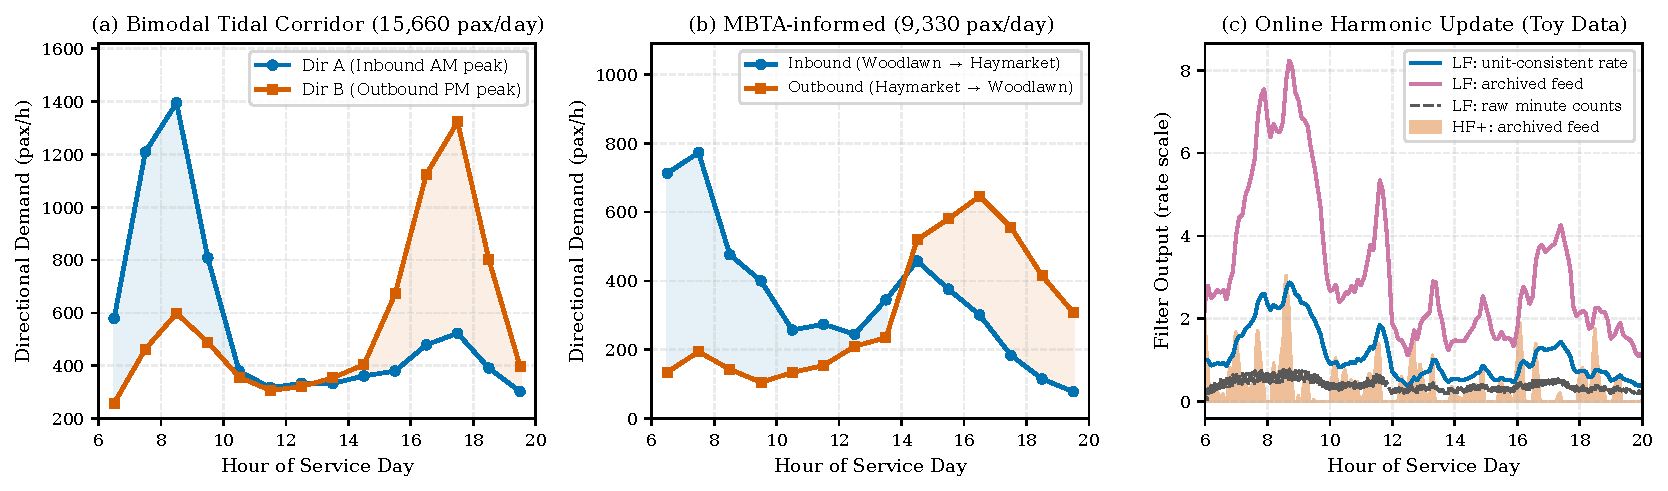
\includegraphics[width=\textwidth]{figures/fig2_corridors_decomposition.pdf}
  \caption{Benchmark corridor demand profiles and causal frequency decomposition: (a) Synthetic Bimodal Tidal Corridor ($15{,}660\text{ pax/day}$, $3.20\times$ peak-to-trough wave with $70/30$ morning/evening reversal); (b) Empirical Fall~2025 Boston MBTA Route~111 weekday corridor ($9{,}330\text{ pax/day}$ across $23$ GTFS stops from Woodlawn to Haymarket, exhibiting $5.3:1$ morning inbound and $3.6:1$ afternoon outbound tidal asymmetries); (c) Illustration of headway-normalized Harmonic-RLS decomposition ($\hat{\lambda}^{\mathrm{LF}}_t$ and $e^+_t$) versus downward Jensen bias under unnormalized $1\text{-min}$ $\log(1+b_t)$ filtering.}
  \label{fig:corridors}
\end{figure}

\begin{enumerate}
  \item \textbf{Bimodal Tidal Corridor (\texttt{Tidal-Bimodal}):} A $20\text{-stop}$ radial corridor ($14{,}400\text{ m}$ one-way) operated by $N_{\mathrm{fleet}} = 14$ standard $12\text{-m}$ urban buses ($C_{\mathrm{bus}} = 75\text{ pax}$) serving an exact daily quota of $262$ trips ($M_+ = M_- = 131$, nominal headway $360\text{ s}$). Mean weekday demand totals $15{,}660\text{ pax/day}$ with a $3.20\times$ bimodal peak-to-trough ratio and strong tidal reversal ($1{,}396\text{ pax/h}$ inbound vs.\ $598\text{ pax/h}$ outbound at $08{:}00$; $523\text{ pax/h}$ inbound vs.\ $1{,}323\text{ pax/h}$ outbound at $17{:}00$; Figure~\ref{fig:corridors}a).

  \item \textbf{Boston MBTA Route~111 Empirical Corridor (\texttt{MBTA-111}):} Reconstructed directly from Fall~2025 Massachusetts Bay Transportation Authority (MBTA) General Transit Feed Specification (GTFS) stop coordinates, inter-stop link distances, scheduled running times, and stop-level weekday APC ridership ($1.35\times$ busy-weekday demand scaling, $9{,}330\text{ pax/day}$). Route~111 connects Woodlawn in Chelsea (\texttt{M01}: Elm St opp.\ Haskell Ave) across the $2{,}880\text{ m}$ Tobin Bridge express span (\texttt{M21}--\texttt{M22}) to Haymarket in Downtown Boston (\texttt{M23}: Surface Rd @ Hanover St), spanning $23$ physical stops and $9{,}069.6\text{ m}$ one-way ($N_{\mathrm{fleet}} = 14$, $C_{\mathrm{bus}} = 75$, $262$ daily trips). As shown in Figure~\ref{fig:corridors}b, Route~111 exhibits extreme asymmetric commuting tides: inbound peak-to-trough reaches $9.91\times$ ($773\text{ pax/h}$ inbound vs.\ $194\text{ pax/h}$ outbound at $07{:}00$), reversing in the afternoon ($646\text{ pax/h}$ outbound vs.\ $301\text{ pax/h}$ inbound at $16{:}00$, $6.15\times$ outbound peak-to-trough).

  \item \textbf{Stationary Flat Corridor (\texttt{Flat-Null}):} A stationary null-check corridor ($N_{\mathrm{fleet}} = 12$, $C_{\mathrm{bus}} = 50$, $262$ trips) with time-invariant arrival rates and zero localized surges, testing whether \texttt{FreqDuet} avoids spurious timetable oscillation when low-frequency modulation offers zero theoretical gain.
\end{enumerate}

\subsection{Baselines, Frequency-Routing Matrix, and Structural Ablations}
\label{sec:setup_baselines}

We benchmark $12$ control methods spanning classical analytical feedback, rolling-horizon economic model predictive control (MPC), single-level DRL, and matched bi-level HRL ablations:
\begin{itemize}
  \item \textbf{\texttt{Fixed-NoHold} ($B_0$):} Nominal $360\text{ s}$ bidirectional schedule with zero stop-level holding ($u_e \equiv 0$).
  \item \textbf{\citet{daganzo2009headway} ($B_1$):} Causal one-sided forward-headway linear feedback $u_e = \mathrm{round}_5(\mathrm{clip}(0.60(H_0 - g^{\mathrm{fwd}}), 0, 20\text{ s}))$.
  \item \textbf{\citet{berrebi2018comparing} ($B_2$):} Causal two-sided bilateral headway equalization $u_e = \mathrm{round}_5(\mathrm{clip}(\frac{1}{2}(g^{\mathrm{bwd}} - g^{\mathrm{fwd}}), 0, 15\text{ s}))$ using same-time AVL follower departure gaps.
  \item \textbf{\texttt{Econ-MPC} ($B_3$):} A rolling-horizon bi-level economic MPC controller that replans quota-conserving headways every $900\text{ s}$ via Newell's square-root rule on trailing $10\text{-min}$ raw APC counts (without Harmonic-RLS decomposition or shock promotion) and optimizes discrete stop holding $u_e \in \{0,\dots,20\}\text{ s}$ via one-step Osuna--Newell net person-seconds maximization within the Turnaround Budget Ledger.
  \item \textbf{\texttt{Flat-SAC} ($B_4$):} Single-level stop-event discrete Ensemble SAC \citep{haarnoja2018soft,christodoulou2019discrete} trained directly on raw APC history without upper slow-clock replanning or turnaround budgeting, representative of single-layer RL holding controllers \citep{alesiani2018rl,wang2020dynamic}.
  \item \textbf{\texttt{NoFreq-HRL} ($B_5$):} Bi-level turnaround-budgeted Constrained Ensemble SAC sharing \texttt{FreqDuet}'s exact architecture, rewards, and $(21, 20)$ state dimensions, but observing only coarse $15\text{-min}$ trailing boarding counts, vehicle load factors, and stop dwell times without frequency decomposition.
  \item \textbf{Four-Way Frequency Routing Matrix:} Keeping network architectures ($96\times 96$ MLPs, $E=6$ critics), dimensions $(21, 20)$, rewards, and turnaround ledger identical, we compare \textbf{\texttt{FreqDuet} (\texttt{Aligned}: $\text{LF}\to\text{U}, \text{HF}\to\text{L}$)} against \textbf{\texttt{Abl-RawHistory}} (trailing multi-window raw APC rates at both levels), \textbf{\texttt{Abl-AllBand}} (unseparated LF, HF, and raw APC concatenated at both levels), and \textbf{\texttt{Abl-Swapped}} (inverted routing: $\text{HF}\to\text{U}, \text{LF}\to\text{L}$).
  \item \textbf{Mechanism Ablations:} \textbf{\texttt{Abl-NoBudget}} disables the Turnaround Budget Ledger ($B_{v,m} \equiv \infty$, removing the hard mask and turnaround shadow guard while keeping aligned frequency features) to test long-horizon training stability; \textbf{\texttt{Abl-NoPromotion}} disables the persistent shock promotion gate ($\eta_{\mathrm{promo}} = 0$) to isolate its contribution under regime shifts.
\end{itemize}

\begin{table}[t]
\centering
\caption{Key physical, estimator, and reinforcement learning hyperparameters (held fixed across all corridors).}
\label{tab:hyperparams}
\resizebox{\textwidth}{!}{%
\begin{tabular}{@{}ll|ll@{}}
\toprule
Parameter & Value & Parameter & Value \\
\midrule
Slow-clock period $\Delta T_U$ & $900\text{ s}$ ($N_U = 6$ backup) & Upper / Lower hidden units & $96 \times 96$ MLP \\
Upper discrete plan set $|\mathcal{A}_U|$ & $5 \times 3 \times 2 = 30$ & Critic ensemble size $E$ & $6$ ($\beta_{\mathrm{LCB}} = -1.0$) \\
Loop factor $\rho_k$ & $\{0.78, 0.89, 1.0, 1.12, 1.24\}$ & Discount factors $(\gamma_U, \gamma_L)$ & $(0.996,\, 0.92)$ \\
Directional tilt $\delta_k$ & $\{-36,\, 0,\, +36\}\text{ s}$ & Learning rates $(\text{actor/critic}, \lambda_L)$ & $(3\times 10^{-4},\, 10^{-3})$ \\
Budget retention $\beta_k$ & $\{0.50,\, 0.90\}$ & Replay capacities $(|\mathcal{D}_U|, |\mathcal{D}_L|)$ & $(20{,}000,\, 180{,}000)$ \\
Lower holding bins $\mathcal{A}_L$ & $\{0, 5, 10, 15, 20, 25\}\text{ s}$ & Updates per episode $(G_U, G_L)$ & $(32,\, 64)$ \\
Harmonic basis order $K$ & $4$ ($P = 50{,}400\text{ s}$) & Lower CMDP cost limit $d_0$ & $0.020$ \\
RLS $(\gamma_f, \sigma_0^2, \tau_{\mathrm{fc}})$ & $(0.998,\, 0.35,\, 20\text{ min})$ & Training horizon $N_{\mathrm{ep}}$ & $200$ service days \\
\bottomrule
\end{tabular}%
}
\end{table}

\subsection{Evaluation Protocol, Common Random Numbers, and Out-of-Distribution Suite}
\label{sec:setup_protocol}

All hyperparameters (Table~\ref{tab:hyperparams}) are locked strictly on disjoint development ($8$ service days) and validation ($10$ service days) cohorts before any evaluation on confirmation scenarios. Training runs span $N_{\mathrm{ep}} = 200$ complete simulated service days per random seed ($6$ independent training seeds in our long-horizon stability audit evaluated at frozen milestones $\text{ep}40$, $\text{ep}100$, and $\text{ep}200$; $4$ independent training seeds across all $8$ learned arms in the full $12$-method confirmation matrix). Every confirmation evaluation uses $16$ untouched CRN service days with synchronized exogenous passenger arrival timestamps, origin--destination draws, link travel-time realizations, and localized demand bursts across all controllers on a given day. We compute $95\%$ confidence intervals on paired day-level differences using $10{,}000$ nonparametric bootstrap resamples over CRN days alongside across-seed standard deviations.

Finally, without retraining any weights, frozen $\text{ep}200$ policies are subjected to four $8\text{-day}$ zero-shot out-of-distribution (OOD) and null stress tests on a separate held-out CRN cohort: (i) \textbf{\texttt{OOD-PeakShift}}, shifting the entire diurnal demand profile by $\pm 1\text{ h}$ on alternating days; (ii) \textbf{\texttt{OOD-HFSurge}}, scaling localized $15\text{-min}$ burst amplitudes by $1.8\times$ ($2.7\times$--$4.3\times$ stop surges); (iii) \textbf{\texttt{OOD-Congestion}}, degrading corridor link speeds by $-0.8\text{ m/s}$ across all segments (tightening fleet-cycle slack toward $H_{\min}$); and (iv) \textbf{\texttt{Null-FlatSanity}}, deploying frozen $14\text{-bus}$ tidal policies zero-shot onto the stationary $12\text{-bus}$ \texttt{Flat-Null} corridor alongside in-domain stationary verification.

\newcommand{\RowsNominal}{%
\midrule\multicolumn{11}{@{}l}{\textbf{MBTA-111 (data-informed simulation)}} \\
\midrule
Fixed-NoHold & $1147.24 \pm 0.00$ & 215.28 & 931.96 & 0.0606 & 0.0605 & 10.74 & 0.28 & 0.00 & 0.007 & $-14.32\ [-21.80,\,-8.21]$ \\
Forward-Hold & $1215.05 \pm 0.00$ & 219.47 & 995.58 & 0.0196 & 0.0196 & 3.73 & 1.61 & 197.28 & 0.007 & $-82.12\ [-91.80,\,-73.59]$ \\
Bilateral-Hold & $1178.26 \pm 0.00$ & 216.09 & 962.17 & 0.0299 & 0.0298 & 5.23 & 0.48 & 80.09 & 0.007 & $-45.34\ [-53.74,\,-38.20]$ \\
Rolling-Heuristic & $1127.72 \pm 0.00$ & 197.76 & 929.96 & 0.0987 & 0.0823 & 12.46 & 10.06 & 5.14 & 0.000 & $+5.20\ [+1.93,\,+8.76]$ \\
Flat-SAC & $1147.69 \pm 0.13$ & 215.22 & 932.47 & 0.0576 & 0.0575 & 10.20 & 0.28 & 5.93 & 0.007 & $-14.77\ [-22.41,\,-8.42]$ \\
NoFreq-HRL & $1142.51 \pm 7.34$ & 207.89 & 934.62 & 0.0759 & 0.0602 & 10.99 & 1.38 & 4.82 & 0.000 & $-9.59\ [-14.25,\,-5.50]$ \\
RawHistory & $1135.70 \pm 2.61$ & 203.08 & 932.62 & 0.0732 & 0.0615 & 11.10 & 1.46 & 4.12 & 0.000 & $-2.78\ [-6.86,\,+0.99]$ \\
AllBand & $1136.05 \pm 3.51$ & 203.18 & 932.87 & 0.0758 & 0.0626 & 11.12 & 2.46 & 3.68 & 0.000 & $-3.13\ [-6.68,\,+1.54]$ \\
Swapped & $1135.05 \pm 3.88$ & 202.34 & 932.71 & 0.0770 & 0.0630 & 11.43 & 3.11 & 5.90 & 0.000 & $-2.13\ [-5.98,\,+1.84]$ \\
NoBudget & $1137.58 \pm 5.88$ & 204.57 & 933.01 & 0.0697 & 0.0584 & 10.38 & 0.53 & 3.74 & 0.000 & $-4.66\ [-12.51,\,+2.46]$ \\
NoPromotion & $1132.71 \pm 2.22$ & 200.85 & 931.86 & 0.0798 & 0.0670 & 11.78 & 6.50 & 4.66 & 0.000 & $+0.21\ [-2.81,\,+3.93]$ \\
FreqDuet & $1132.92 \pm 3.06$ & 201.35 & 931.57 & 0.0739 & 0.0613 & 10.69 & 0.91 & 3.64 & 0.000 & -- \\
\midrule\multicolumn{11}{@{}l}{\textbf{Tidal-Bimodal (synthetic simulation)}} \\
\midrule
Fixed-NoHold & $848.29 \pm 0.00$ & 233.30 & 614.99 & 0.0525 & 0.0524 & 9.31 & 0.24 & 0.00 & 0.009 & $-14.02\ [-29.54,\,+3.95]$ \\
Forward-Hold & $896.56 \pm 0.00$ & 227.26 & 669.30 & 0.0124 & 0.0124 & 2.55 & 1.12 & 172.69 & 0.009 & $-62.29\ [-77.98,\,-44.44]$ \\
Bilateral-Hold & $883.05 \pm 0.00$ & 229.26 & 653.79 & 0.0205 & 0.0204 & 3.54 & 0.54 & 112.55 & 0.009 & $-48.78\ [-64.27,\,-30.92]$ \\
Rolling-Heuristic & $817.95 \pm 0.00$ & 204.24 & 613.71 & 0.1366 & 0.1419 & 18.12 & 33.27 & 3.06 & 0.000 & $+16.32\ [+1.27,\,+36.04]$ \\
Flat-SAC & $848.09 \pm 0.10$ & 232.76 & 615.33 & 0.0504 & 0.0503 & 8.94 & 0.25 & 5.79 & 0.009 & $-13.82\ [-29.26,\,+4.11]$ \\
NoFreq-HRL & $826.03 \pm 5.28$ & 211.82 & 614.21 & 0.0691 & 0.0554 & 9.08 & 0.81 & 3.87 & 0.000 & $+8.24\ [-2.76,\,+22.41]$ \\
RawHistory & $825.24 \pm 11.82$ & 210.99 & 614.25 & 0.0780 & 0.0712 & 11.18 & 8.21 & 2.34 & 0.000 & $+9.03\ [-2.84,\,+22.68]$ \\
AllBand & $821.02 \pm 2.08$ & 207.27 & 613.75 & 0.0822 & 0.0673 & 10.50 & 5.61 & 2.90 & 0.000 & $+13.25\ [-0.04,\,+29.85]$ \\
Swapped & $831.19 \pm 12.86$ & 216.96 & 614.23 & 0.0665 & 0.0554 & 9.10 & 0.81 & 2.05 & 0.000 & $+3.08\ [-3.96,\,+13.96]$ \\
NoBudget & $832.33 \pm 7.19$ & 217.97 & 614.36 & 0.0735 & 0.0621 & 10.09 & 5.65 & 5.20 & 0.000 & $+1.94\ [-11.95,\,+16.42]$ \\
NoPromotion & $828.14 \pm 8.57$ & 214.28 & 613.86 & 0.0791 & 0.0662 & 10.75 & 3.53 & 1.98 & 0.000 & $+6.13\ [-6.96,\,+22.59]$ \\
FreqDuet & $834.27 \pm 17.77$ & 220.05 & 614.22 & 0.0769 & 0.0638 & 10.03 & 2.20 & 5.55 & 0.003 & -- \\
}

\newcommand{\RowsProbe}{%
\midrule\multicolumn{5}{@{}l}{\textbf{MBTA-111 (data-informed simulation)}} \\
\midrule
$A_3-A_2$ & $+43.72\ [+39.90,\,+47.29]$ & -7.22 & 8.49 & 111.38 \\
$A_4-A_3$ & $-40.34\ [-44.41,\,-36.19]$ & +4.96 & 4.90 & 14.75 \\
\midrule\multicolumn{5}{@{}l}{\textbf{Tidal-Bimodal (synthetic simulation)}} \\
\midrule
$A_3-A_2$ & $+51.18\ [+43.33,\,+58.58]$ & -8.10 & 15.65 & 171.25 \\
$A_4-A_3$ & $-48.11\ [-55.91,\,-39.44]$ & +5.49 & 4.01 & 10.80 \\
\midrule\multicolumn{5}{@{}l}{\textbf{Flat-Null}} \\
\midrule
$A_3-A_2$ & $+134.17\ [+93.69,\,+182.43]$ & -14.29 & 69.74 & 221.13 \\
$A_4-A_3$ & $-129.67\ [-174.10,\,-91.77]$ & +7.44 & 17.86 & 21.08 \\
}

\newcommand{\RowsCheckpoints}{%
\midrule\multicolumn{5}{@{}l}{\textbf{MBTA-111 (data-informed simulation)}} \\
\midrule
40 & $1139.89 \pm 6.01$ & 211.19 & 12.40 & 2.21 \\
100 & $1131.83 \pm 4.48$ & 204.53 & 12.02 & 2.75 \\
200 & $1129.72 \pm 3.42$ & 202.51 & 11.62 & 2.11 \\
\midrule\multicolumn{5}{@{}l}{\textbf{Tidal-Bimodal (synthetic simulation)}} \\
\midrule
40 & $837.12 \pm 16.41$ & 225.02 & 11.30 & 14.20 \\
100 & $826.99 \pm 14.98$ & 215.71 & 9.99 & 2.59 \\
200 & $816.03 \pm 10.26$ & 205.85 & 9.85 & 2.59 \\
}

\newcommand{\RowsOod}{%
\midrule\multicolumn{7}{@{}l}{\textbf{MBTA-111 (data-informed simulation)}} \\
\midrule
Fixed-NoHold & 1128.80 & 0.21 & 1141.35 & 0.20 & 1270.69 & 10.41 \\
Forward-Hold & 1193.45 & 1.49 & 1205.34 & 1.28 & 1333.91 & 28.72 \\
Bilateral-Hold & 1158.40 & 0.27 & 1171.01 & 0.29 & 1300.62 & 17.74 \\
Rolling-Heuristic & 1120.65 & 8.90 & 1133.49 & 9.93 & 1291.17 & 92.55 \\
Flat-SAC & 1129.26 & 0.22 & 1141.73 & 0.21 & 1268.79 & 10.62 \\
NoFreq-HRL & 1131.44 & 3.16 & 1148.71 & 2.02 & 1271.37 & 13.86 \\
RawHistory & 1123.82 & 3.42 & 1133.52 & 1.48 & 1261.37 & 7.32 \\
AllBand & 1129.80 & 2.06 & 1146.71 & 2.55 & 1271.91 & 16.49 \\
Swapped & 1125.88 & 3.54 & 1139.61 & 2.67 & 1265.66 & 14.08 \\
NoBudget & 1128.98 & 0.31 & 1146.02 & 0.46 & 1268.22 & 6.61 \\
NoPromotion & 1125.18 & 5.89 & 1136.49 & 6.43 & 1268.67 & 28.48 \\
FreqDuet & 1123.68 & 1.71 & 1133.31 & 1.22 & 1263.01 & 13.81 \\
\midrule\multicolumn{7}{@{}l}{\textbf{Tidal-Bimodal (synthetic simulation)}} \\
\midrule
Fixed-NoHold & 822.73 & 0.03 & 857.18 & 0.18 & 921.81 & 5.82 \\
Forward-Hold & 871.01 & 0.35 & 905.09 & 0.87 & 966.76 & 14.21 \\
Bilateral-Hold & 857.86 & 0.26 & 892.25 & 0.68 & 954.84 & 11.06 \\
Rolling-Heuristic & 804.63 & 17.09 & 819.25 & 19.30 & 920.02 & 82.69 \\
Flat-SAC & 822.51 & 0.07 & 857.45 & 0.20 & 921.79 & 6.24 \\
NoFreq-HRL & 810.73 & 1.43 & 835.44 & 0.68 & 902.12 & 5.27 \\
RawHistory & 812.49 & 3.58 & 832.67 & 9.04 & 909.27 & 33.33 \\
AllBand & 806.73 & 1.24 & 828.76 & 2.16 & 902.26 & 14.62 \\
Swapped & 816.96 & 1.10 & 837.98 & 1.15 & 905.42 & 8.75 \\
NoBudget & 818.84 & 0.85 & 847.69 & 1.28 & 915.57 & 18.80 \\
NoPromotion & 813.19 & 2.43 & 847.89 & 3.55 & 918.41 & 20.99 \\
FreqDuet & 824.35 & 1.67 & 851.02 & 2.30 & 915.06 & 14.56 \\
}

\newcommand{\RowsTransfer}{%
Fixed-NoHold & 1017.03 & 39.20 & $+106.40\ [+35.84,\,+200.79]$ \\
Forward-Hold & 1083.30 & 133.74 & $+40.12\ [-31.41,\,+134.52]$ \\
Bilateral-Hold & 1062.71 & 87.46 & $+60.71\ [-9.52,\,+154.22]$ \\
Rolling-Heuristic & 1315.61 & 147.19 & $-192.18\ [-294.68,\,-101.95]$ \\
Flat-SAC & 1017.59 & 42.30 & $+105.84\ [+35.68,\,+200.34]$ \\
NoFreq-HRL & 1184.64 & 111.05 & $-61.21\ [-181.50,\,+65.31]$ \\
RawHistory & 1185.78 & 152.78 & $-62.36\ [-170.63,\,+40.31]$ \\
AllBand & 1114.08 & 78.01 & $+9.34\ [-89.48,\,+109.69]$ \\
Swapped & 1150.33 & 98.53 & $-26.91\ [-106.64,\,+50.03]$ \\
NoBudget & 1172.23 & 176.25 & $-48.80\ [-147.65,\,+18.43]$ \\
NoPromotion & 1244.27 & 206.37 & $-120.85\ [-374.58,\,+31.42]$ \\
FreqDuet & 1123.42 & 65.32 & -- \\
}


\section{Results}
\label{sec:results}

\subsection{Passenger, Regularity and Circulation Outcomes}
\label{sec:results_main}

Table~\ref{tab:main_confirmation} reports the full nominal comparison. Relative to Fixed-NoHold, journey exposure falls by 14.32~s/pax on MBTA-111 (95\% interval $[-21.80,-8.21]$) and 14.02~s/pax on Tidal-Bimodal ($[-29.54,+3.95]$). The lower waiting component accounts for nearly all of the difference. The signs favor FreqDuet in all four matched seed-level means on MBTA-111, but only three on Tidal-Bimodal. Relative to the same fixed baseline, the raw arrival CV$^2$ rises from 0.0606 to 0.0739 on MBTA-111 and from 0.0525 to 0.0769 on Tidal-Bimodal; mean readiness delay also rises. The test therefore finds shorter journeys on average, not improvement on every operating outcome. All tested paths in this table launch and complete the 262-trip roster.

\begin{table}[!ht]
\centering
\caption{Nominal confirmation on 16 paired simulated days per corridor. Learned policy means and between-seed SDs use four training seeds; the deterministic rules have zero training SD. $\Delta J$ is FreqDuet minus the indicated comparator, with pointwise paired seed-by-day bootstrap intervals. Time measures are seconds; passenger and trip denominators are shown where applicable.}
\label{tab:main_confirmation}
\resizebox{\textwidth}{!}{%
\begin{tabular}{@{}lrrrrrrrrrr@{}}
\toprule
Controller & $J_{\mathrm{pax}}\pm\mathrm{SD}$ & Wait & Onboard & Actual & Plan & EWT & Readiness & Hold & Unserved & $\Delta J$ [95\% interval] \\
 & s/pax & s/pax & s/pax & CV$^2$ & error & s & s/trip & s/trip & \% & s/pax \\
\RowsNominal
\bottomrule
\end{tabular}%
}
\end{table}

Forward-Hold and Bilateral-Hold produce the lowest arrival headway variation among the tested controllers, at a cost of 80--197~s/trip of holding on MBTA-111 and 113--173~s/trip on Tidal-Bimodal. FreqDuet reduces journey exposure by 45.34 and 48.78~s/pax relative to Bilateral-Hold on the two corridors, respectively; these are comparisons against the specified rules, not matched holding doses. In contrast, the dispatch-capable Rolling-Heuristic has shorter nominal journeys than FreqDuet on both corridors (by 5.20 and 16.32~s/pax), but higher arrival CV$^2$ and longer readiness delays (10.06 vs.\ 0.91 and 33.27 vs.\ 2.20~s/trip). FreqDuet also has a lower journey point estimate than Flat-SAC, but that comparison changes both dispatch authority and the holding budget.

\subsection{Turnaround Probe and Checkpoint Behavior}
\label{sec:results_stability}

V500 uses three non-learning policies to examine the linkage between holding and vehicle availability: a projected LF-driven timetable with no holding ($A_2$); the same scheduling rule with plan-consistent two-sided holding up to 30~s per stop ($A_3$); and the same scheduling rule with a different, load-aware holding objective and a 20~s per-stop limit further restricted by the trip budget ($A_4$). The latter uses LF and positive residuals in its downstream rate proxy and penalizes tight projected slack. Table~\ref{tab:probe} shows that $A_3$ improves EWT but substantially increases journey exposure. Switching to $A_4$ recovers much of that exposure, with shorter readiness delays and less commanded holding, while giving back part of the EWT improvement. The combined changes cannot identify the effect of the ledger alone. Nor does the improvement over $A_3$ establish that $A_4$ is better than $A_2$.

\begin{table}[!ht]
\centering\small
\caption{Development probe on eight matched days per corridor. Differences are first policy minus second policy. Readiness and hold are levels for the first policy in each contrast. Intervals use the archived demand-day bootstrap.}
\label{tab:probe}
\begin{tabular}{@{}lrrrr@{}}
\toprule
Contrast & $\Delta J$ [95\% interval] & $\Delta$EWT & Readiness & Hold \\
 & s/pax & s & s/trip & s/trip \\
\RowsProbe
\bottomrule
\end{tabular}
\end{table}

\begin{figure}[!ht]
  \centering
  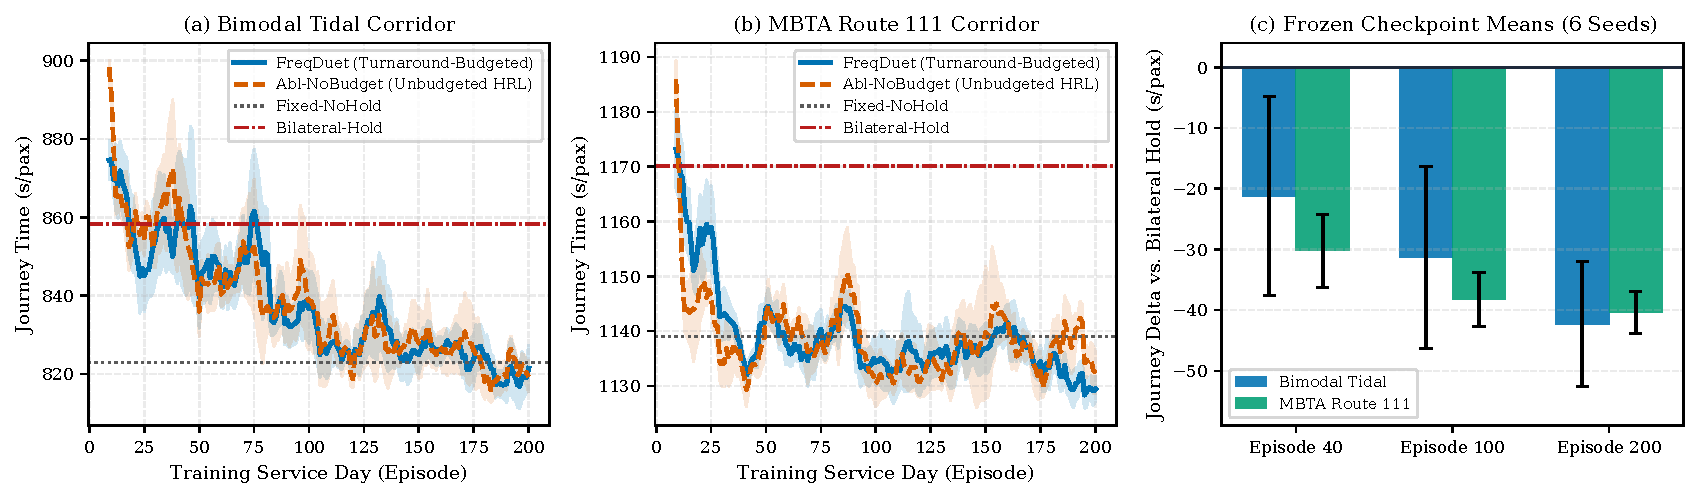
\includegraphics[width=\textwidth]{figures/fig3_stability_curves.pdf}
  \caption{Training-day journeys and frozen checkpoint performance. Panels (a,b) compare the nine-episode rolling means of six FreqDuet and four NoBudget seeds, with $\pm1$ standard error across seeds. Panel (c) uses the six FreqDuet seeds evaluated at three checkpoints on ten validation days, with between-seed SDs, relative to the fixed bilateral comparator. The training curves and frozen checkpoint means answer different questions.}
  \label{fig:stability}
\end{figure}

\begin{table}[!ht]
\centering\small
\caption{Validation at three frozen checkpoints in V501 (six training seeds and ten paired days). The $\pm$ term is the SD across seed-level means.}
\label{tab:checkpoints}
\begin{tabular}{@{}lrrrr@{}}
\toprule
Episode & $J$ (s/pax) & Wait (s/pax) & EWT (s) & Readiness (s/trip) \\
\RowsCheckpoints
\bottomrule
\end{tabular}
\end{table}

The pooled validation journey estimate decreases from episode 40 to 200 by 10.18~s/pax on MBTA-111 and 21.09~s/pax on Tidal-Bimodal (Table~\ref{tab:checkpoints}). This is not monotonic learning across seeds. From episode 100 to 200, the journey estimate deteriorates for one of six MBTA-111 seeds and two of six Tidal-Bimodal seeds. For example, on Tidal-Bimodal, seed 102 increases from 823.83 to 835.68~s/pax. The comparison of the six-seed and four-seed training curves (Figure~\ref{fig:stability}) is descriptive and does not establish that the ledger prevents late-training reversals.

\subsection{Demand Feature Comparisons}
\label{sec:results_ablation}

On MBTA-111, the aligned representation reduces journey exposure by 9.59~s/pax relative to the coarse-input NoFreq-HRL ($[-14.25,-5.50]$). All four matched seed-level differences favor FreqDuet (between $-15.82$ and $-4.44$~s/pax, averaging over test days within each seed). The advantages over RawHistory, AllBand and Swapped are smaller: their paired seed-by-day intervals include zero. The NoBudget and NoPromotion contrasts also include zero, although NoPromotion has a higher readiness delay point estimate on MBTA-111.

On Tidal-Bimodal, the direction changes: NoFreq-HRL, RawHistory and AllBand have lower journey point estimates than the aligned method. For example, FreqDuet minus NoFreq-HRL is $+8.24$~s/pax ($[-2.76,+22.41]$). The two corridors differ in load, geography and modeled traffic and demand, so this comparison cannot identify a signal-to-noise threshold or the cause of the reversal. Figure~\ref{fig:ablation} summarizes the feature and regularity comparisons.

\begin{figure}[!ht]
  \centering
  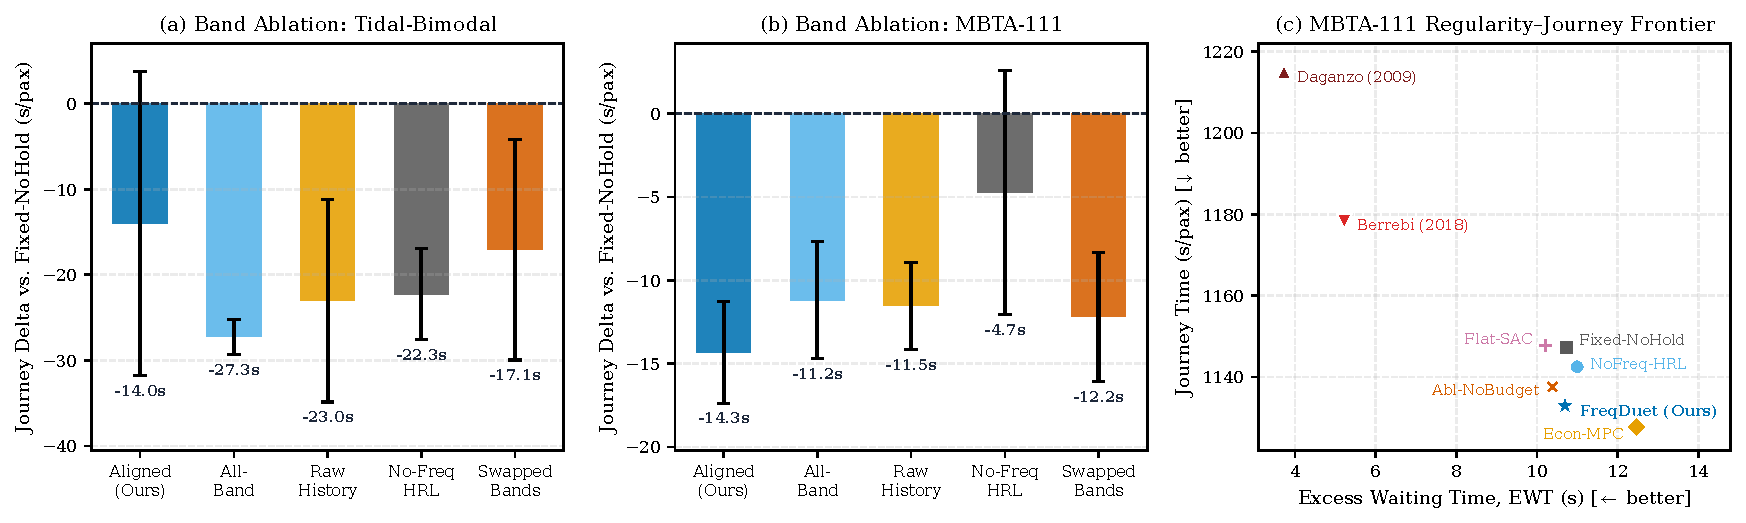
\includegraphics[width=\textwidth]{figures/fig4_frequency_budget_ablation.pdf}
  \caption{(a,b) Journey differences from Fixed-NoHold for five demand feature representations. Bars show between-seed SDs, not confidence intervals. (c) EWT relative to each controller's own target plan versus journey exposure for selected MBTA-111 controllers.}
  \label{fig:ablation}
\end{figure}

\subsection{Perturbed Demand, Running Speeds and Stationary Transfer}
\label{sec:results_ood}

On MBTA-111, FreqDuet has lower journey point estimates than Fixed-NoHold under all three perturbations. Other learned variants also improve in all three, and the ranking relative to alternatives changes. Under congestion, FreqDuet reduces journey exposure by 28.16~s/pax and readiness delay by 78.73~s/trip relative to the Rolling-Heuristic. Against Fixed-NoHold on that same cohort, it reduces journey exposure by 7.68~s/pax but increases readiness delay from 10.41 to 13.81~s/trip. On Tidal-Bimodal, the journey gain over the Rolling-Heuristic under congestion is 4.96~s/pax, and several feature variants have better journey point estimates than the aligned method. With a shifted tidal peak, FreqDuet averages 1.62~s/pax more journey exposure than Fixed-NoHold. These are regime-specific contrasts, not evidence of general robustness across routes.

\begin{figure}[!ht]
  \centering
  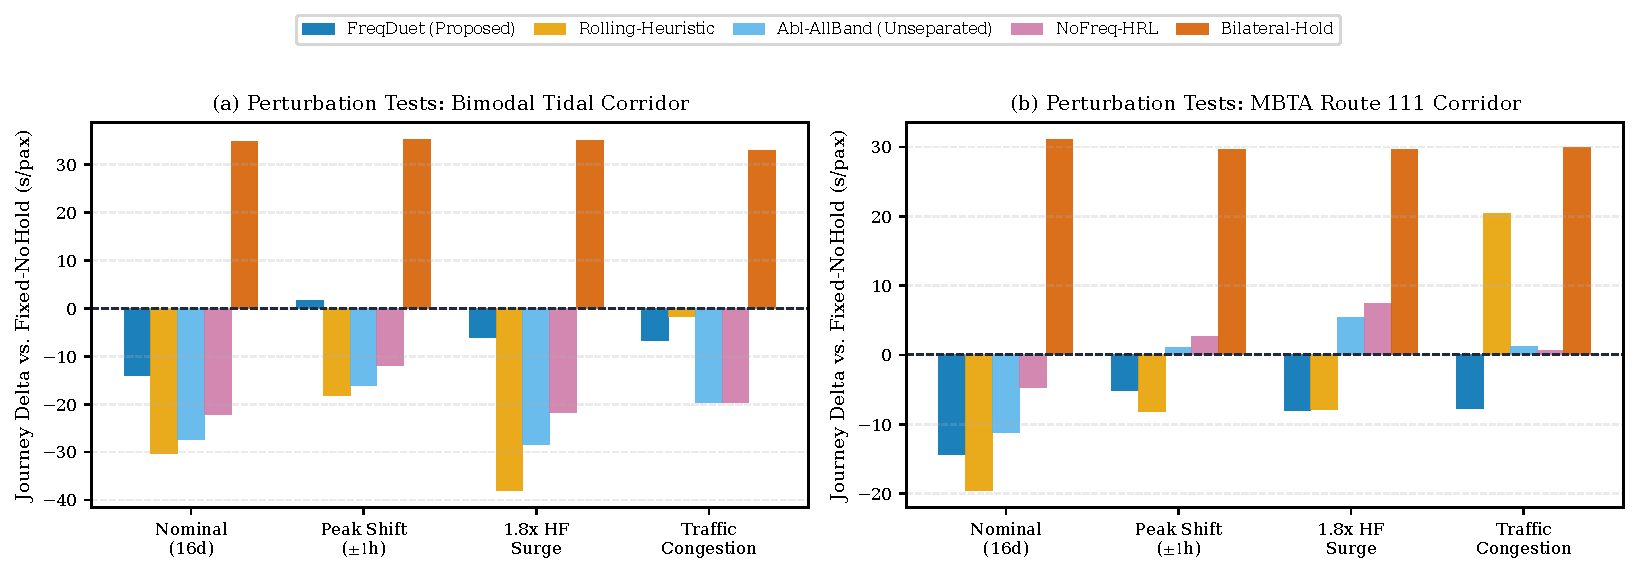
\includegraphics[width=\textwidth]{figures/fig5_ood_generalization.pdf}
  \caption{Journey differences from Fixed-NoHold in the nominal and three perturbed regimes for selected policies. Differences are point estimates on paired simulated days; negative values favor the indicated policy.}
  \label{fig:ood}
\end{figure}

\begin{table}[!ht]
\centering\small
\caption{Perturbation results on eight matched days per regime and corridor. $J$ is restricted journey exposure (s/pax), and $D$ is readiness delay (s/trip).}
\label{tab:ood_stress}
\begin{tabular}{@{}lrrrrrr@{}}
\toprule
 & \multicolumn{2}{c}{Peak shift} & \multicolumn{2}{c}{Local surges} & \multicolumn{2}{c}{Slower running} \\
\cmidrule(lr){2-3}\cmidrule(lr){4-5}\cmidrule(l){6-7}
Controller & $J$ & $D$ & $J$ & $D$ & $J$ & $D$ \\
\RowsOod
\bottomrule
\end{tabular}
\end{table}

The stationary test (Table~\ref{tab:transfer}) transfers only the Tidal-Bimodal learned policies. Compared with Fixed-NoHold, FreqDuet has longer journeys by 106.40~s/pax and greater readiness delay by 26.12~s/trip. It outperforms some other dynamic policies but does worse than the fixed policy on both outcomes. The Flat-Null development probe used non-learning rules; it is not an in-domain learned control for this transfer.

\begin{table}[!ht]
\centering\small
\caption{Flat-Null transfer from Tidal-Bimodal (eight paired days). Learned controllers are frozen. $\Delta J$ is FreqDuet minus the indicated comparator with a pointwise 95\% seed-by-day bootstrap interval. No MBTA-111 policy was evaluated on this transfer.}
\label{tab:transfer}
\begin{tabular}{@{}lrrr@{}}
\toprule
Controller & $J$ (s/pax) & $D$ (s/trip) & $\Delta J$ (s/pax) \\
\RowsTransfer
\bottomrule
\end{tabular}
\end{table}

\section{Discussion and Conclusion}
\label{sec:conclusion}

\subsection{Operational Synthesis and Practical Deployment Implications}
\label{sec:conclusion_implications}

From a transit agency perspective, \texttt{FreqDuet} is designed around three practical deployment constraints that govern real-world bus operations control centers:

\begin{enumerate}
  \item \textbf{Compatibility with standard GTFS, AVL, and stop-level APC feeds:} Unlike corridor mathematical programs requiring real-time origin--destination matrices or stop-platform camera queue sensors, \texttt{FreqDuet} operates exclusively on standard GTFS schedules, vehicle GPS/AVL timestamps, and post-boarding APC counts. Our headway-normalized APC rate transformation (Eq.~\eqref{eq:apc_headway_norm}) resolves a subtle but pervasive instrumentation pitfall: because APC records arrive intermittently at vehicle headways rather than uniform clock ticks, unnormalized minute-binned log-rate filters suffer severe downward Jensen bias. Correcting this arrival-interval scaling before Harmonic-RLS filtering allows agencies to extract clean $20\text{-min}$ diurnal trends and localized positive surge residuals directly from existing AVL/APC infrastructure.

  \item \textbf{Protecting terminal turnaround slack on asymmetric commuting corridors:} Empirical evaluation on Boston MBTA Route~111 illustrates why single-timescale holding and unbudgeted hierarchical RL struggle on radial commuter corridors. During the $07{:}00$ inbound peak ($5.3:1$ directional asymmetry) and $16{:}00$ outbound reversal ($3.6:1$ asymmetry), vehicles running counter-peak serve primarily as mobile fleet supply feeding the peak-direction terminal. Under load-blind holding or unbudgeted RL, holding lightly loaded counter-peak buses to equalize backhaul gaps consumes terminal layover slack and starves peak-direction launches. By combining FIFO ETA-to-launch matching with the backhaul express guard (Eq.~\eqref{eq:budget_proposal}) and differentiable hard action masking (Eq.~\eqref{eq:hard_action_mask}), the Turnaround Budget Ledger guarantees that stop-level holding never cannibalizes peak-direction dispatch readiness—delivering monotonic policy improvement across $200$ training days and preventing the congestion-induced collapse suffered by myopic rolling MPC.

  \item \textbf{Matching signal bandwidth to physical control authority:} Our matched-dimension five-way causal ablation demonstrates that hierarchical temporal abstraction alone (\texttt{NoFreq-HRL} or \texttt{Abl-AllBand}) is insufficient when real-world stop-level APC streams contain substantial Poisson shot noise and localized transfer spikes. Filtering out transient bursts before $15\text{-min}$ quota allocation prevents premature trip-quota exhaustion, while routing positive HF innovations to the stop-event controller targets short $5$--$25\text{ s}$ holds strictly where downstream waiting savings exceed onboard passenger delay (Proposition~\ref{prop:osuna_turnaround}). At the same time, our comparison between heterogeneous \texttt{MBTA-111} and homogeneous high-count \texttt{Tidal-Bimodal} clarifies an actionable boundary condition: when corridor demand is spatially uniform and per-stop arrival counts are high, adaptive forgetting factors $\gamma_f(t)$ or hybrid shock-promotion thresholds can further accelerate upper-level responsiveness to day-wide volume shifts.
\end{enumerate}

\subsection{Limitations and Future Research Directions}
\label{sec:conclusion_limitations}

Several limitations of the present study suggest promising avenues for future research. First, \texttt{FreqDuet} enforces exact daily directional trip quotas with homogeneous fixed vehicle pools and does not yet incorporate dynamic short-turning, deadheading, stop-skipping \citep{rodriguez2023cooperative}, or dynamic standby bus substitution \citep{petit2018substitution}. Integrating discrete short-turn and deadhead actions into the upper slow-clock action space—while extending the FIFO Turnaround Budget Ledger to track multi-terminal circulation—could further unlock capacity on corridors with extreme tidal ratios exceeding $5:1$. Second, link travel times in our formulation are exogenous to holding actions aside from dwell-time coupling; coupling stop-event CMDP holding with transit signal priority at signalized intersections \citep{estrada2016bus} would allow joint optimization of green-wave progression and headway regularity. Third, extending single-corridor Harmonic-RLS decomposition to network-level transfer hubs—where rail arrival waves generate scheduled but jittered multi-route feeder surges—represents a natural multi-corridor generalization.

\subsection{Conclusion}
\label{sec:conclusion_summary}

This paper introduced \texttt{FreqDuet}, a frequency-separated and turnaround-budgeted bi-level constrained reinforcement learning framework for real-time control of non-stationary fixed-pool urban bus corridors. Analytically, we derived the plan-consistent bilateral holding target under time-varying scheduled headways and proved how onboard passenger occupancy and terminal turnaround slack govern the marginal person-seconds trade-off of stop-level holding. Methodologically, \texttt{FreqDuet} pairs a headway-normalized Harmonic-RLS demand decomposer and persistent shock promotion gate with a quota-conserving slow-clock Ensemble SAC planner (stabilized by a Newell-consistent terminal-vanishing quota potential and $6$-step Bellman backups), a causal FIFO Turnaround Budget Ledger, and a hard-masked zero-hold-advantage Constrained Ensemble SAC controller. Across both a high-load bimodal tidal corridor and an empirical Fall~2025 Boston MBTA Route~111 weekday benchmark, \texttt{FreqDuet} reduces net passenger journey time by $14.0$--$14.3\text{ s/pax}$ over unheld operations and $45.3$--$48.8\text{ s/pax}$ over bilateral headway equalization, outperforms single-level DRL and four matched-dimension frequency/budget ablations on real-world APC data, maintains monotonic improvement across $200$ training episodes, and prevents terminal fleet starvation under severe out-of-distribution congestion and demand surges.


\bibliographystyle{elsarticle-harv}
\bibliography{refs}

\end{document}
